\documentclass[a4paper, 12pt]{article}

%%%%%%%%%%%%%%%%%%% Packages

\usepackage[french, english]{babel}
\usepackage[noheader]{packages/sleek}
\usepackage{packages/sleek-title}
\usepackage{packages/sleek-theorems}
\usepackage{subcaption}

%%%%%%%%%%%%%%%%%%% Titlepage

\logo{./resources/pdf/logo.pdf}
\institute{University of Liège}
\title{Big Data - Review 5}
\subtitle{Renewable Energy Production Forecast}
\author{Yann \textsc{Claes}\\Gaspard \textsc{Lambrechts}\\François \textsc{Rozet}}
%\context{}
\date{\today}

%%%%%%%%%%%%%%%%%%% Bibliography

\addbibresource{./resources/bib/references.bib}

%%%%%%%%%%%%%%%%%%%

\begin{document}
\maketitle

\section{Photovoltaic production}
\subsection{Tests of the provincial model}
As a reminder, the output power is computed in the following way:
\begin{equation*}
    P = \eta I A
\end{equation*}
with $A = peak\_power * area\_peak$, where $peak\_power$ is the installed power in the province of Liège and $area\_peak$ is an approximation of the area of panels per unit of installed power.

A test procedure has been conducted to evaluate the posterior model built using PyStan. The procedure is the following: fit the parameters ($\eta$, $I$, $area\_peak$, $peak\_power$) on measures collected by Elia for the last 7 days, using a normal distribution, and predict the produced power for the following day, using a normal distribution as well. This seemed to yield very good results for some days, but also more moderate results for other days, mostly depending on the shape of the irradiance curve.

We decided to apply this procedure to the whole 2019 year.

In order to have another line of comparison, we decided to introduce 2 very simple baseline models: 
\begin{itemize}
    \item Predict for day $D+1$ the production measured at day $D$
    \item Predict for day $D+1$ the average of the measured productions for the last 7 days
\end{itemize}

Finally, we have also computed the metrics for Elia's predictions. This way, we can have an insight about wether or not our predictions are sensitive. As for the last review, the computed metrics are the mean-square error and the root mean-square error.

Results to these tests can be found in Table \ref{tab:pv_metrics_meas} .Note that these tests have been conducted using irradiance measurements, and not irradiance forecasts, for the sole reason that we do not have access to past irradiance forecasts. Hence, it is likely that our predictions in these tests will be better than what we would have obtained using forecast measures. Furthermore, as for the previous review, these metrics have been computed without taking night observations into account, since they would give a biased estimate of the true metrics values. 
\begin{table}[h]
	\centering
    \begin{tabular}{l|c|c}
                        & MSE      & RMSE   \\ \hline
        Prior model     & 682.451  & 23.617 \\ \hline
        Posterior model & 469.842  & 19.398 \\ \hline
        Baseline 1      & 2361.555 & 40.390 \\ \hline
        Baseline 2      & 2003.102 & 39.617 \\ \hline
        Elia's forecast & 423.539  & 17.891
    \end{tabular}
    \noskipcaption{Mean of the MSE and RMSE (MW) for 2019.}
    \label{tab:pv_metrics_meas}
\end{table}
From these results, we can see that our posterior model seems to perform better than both baseline models, and is also better than our prior model. Elia's forecasts are obviously better, but we can notice that, on average, we are quite close to their results.

\subsection{Introduction of forecast measures}
Forecast measures have been collected from April 2nd (10:30 UTC) up to April 21\up{st} (11:00 UTC). However, since Elia's measures are only available up to the present day, we have decided to conduct the procedure on 10 days, starting the predictions from April 3\up{rd}.

As for the previous section, we decided to compare our prior and posterior models to Elia's predictions as well as the abovedefined baselines. The results can be found in Table \ref{tab:pv_metrics_for}.
\begin{table}[h]
	\centering
    \begin{tabular}{l|c|c}
                        & MSE      & RMSE   \\ \hline
        Prior model     & 2797.307  & 50.281 \\ \hline
        Posterior model & 1385.751  & 32.594 \\ \hline
        Baseline 1      & 1294.487 & 24.136 \\ \hline
        Baseline 2      & 1039.525 & 27.152 \\ \hline
        Elia's forecast & 292.916  & 15.219
    \end{tabular}
    \noskipcaption{Mean of the MSE and RMSE (MW) for 10 days.}
    \label{tab:pv_metrics_for}
\end{table}
Again, we see that our posterior model performs way better than our prior model. Nevertheless, this time, we see that the baseline models perform even with our posterior model. This can be explained by taking a glance at the measures made by Elia for the considered forecast period. Indeed, by looking at Figure \ref{fig:prior_model}, we see that Elia's measurements are quite the same throughout the forecast period. Hence, in that case, taking the measured production of the previous day/the average over the last 7 days is indeed a good approximation.
\begin{figure}[H]
    \centering
    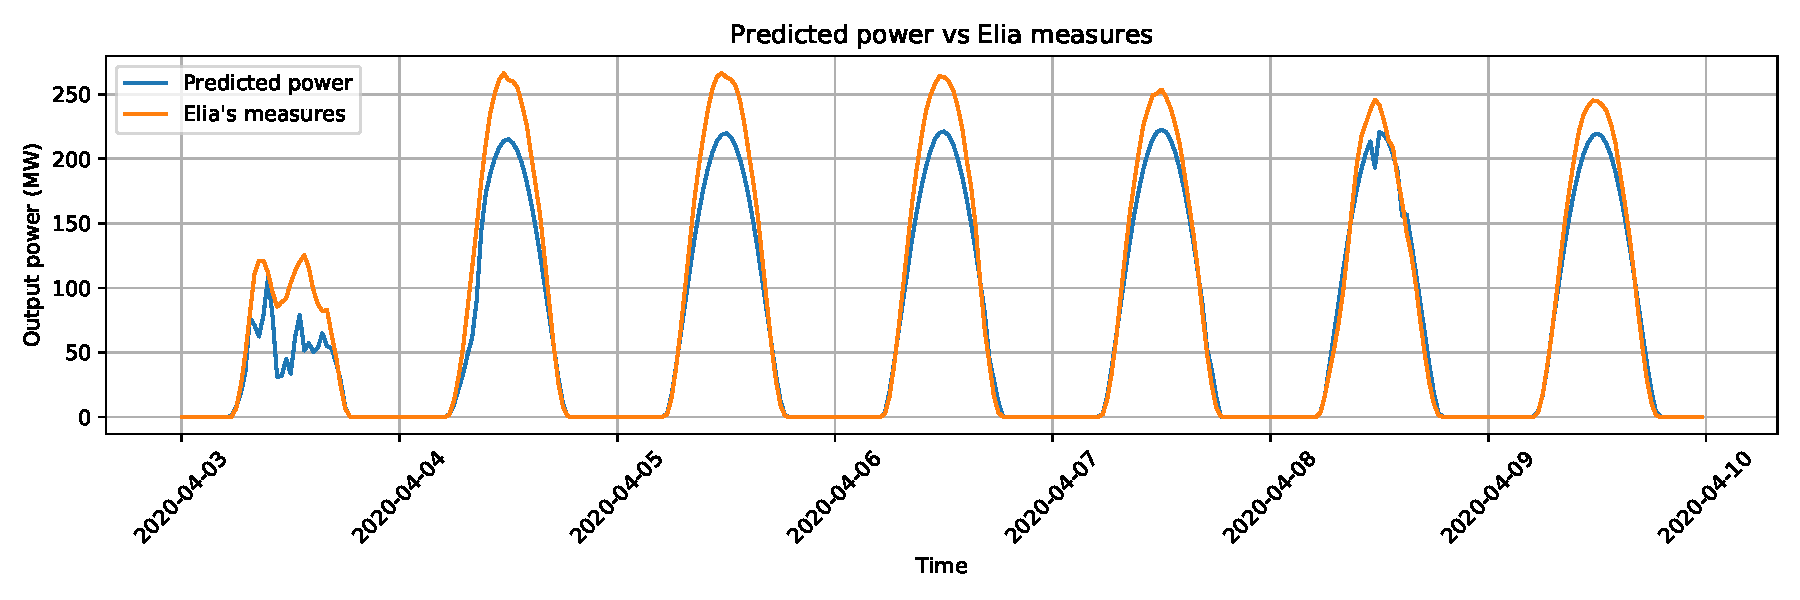
\includegraphics[width=\textwidth]{resources/pdf/province_naive_03-04-2020.pdf}
    \noskipcaption{Comparison between Elia's measurements and the prior model (using irradiance measurements).}
    \label{fig:prior_model}
\end{figure}

We can verify that by looking at the prediction made for April 5\up{th}, depicted on Figure \ref{fig:naive_posterior_5_april}, \ref{fig:base_1_elia_5_april} and \ref{fig:base_2_elia_5_april}.

\begin{figure}[H]
    \centering
    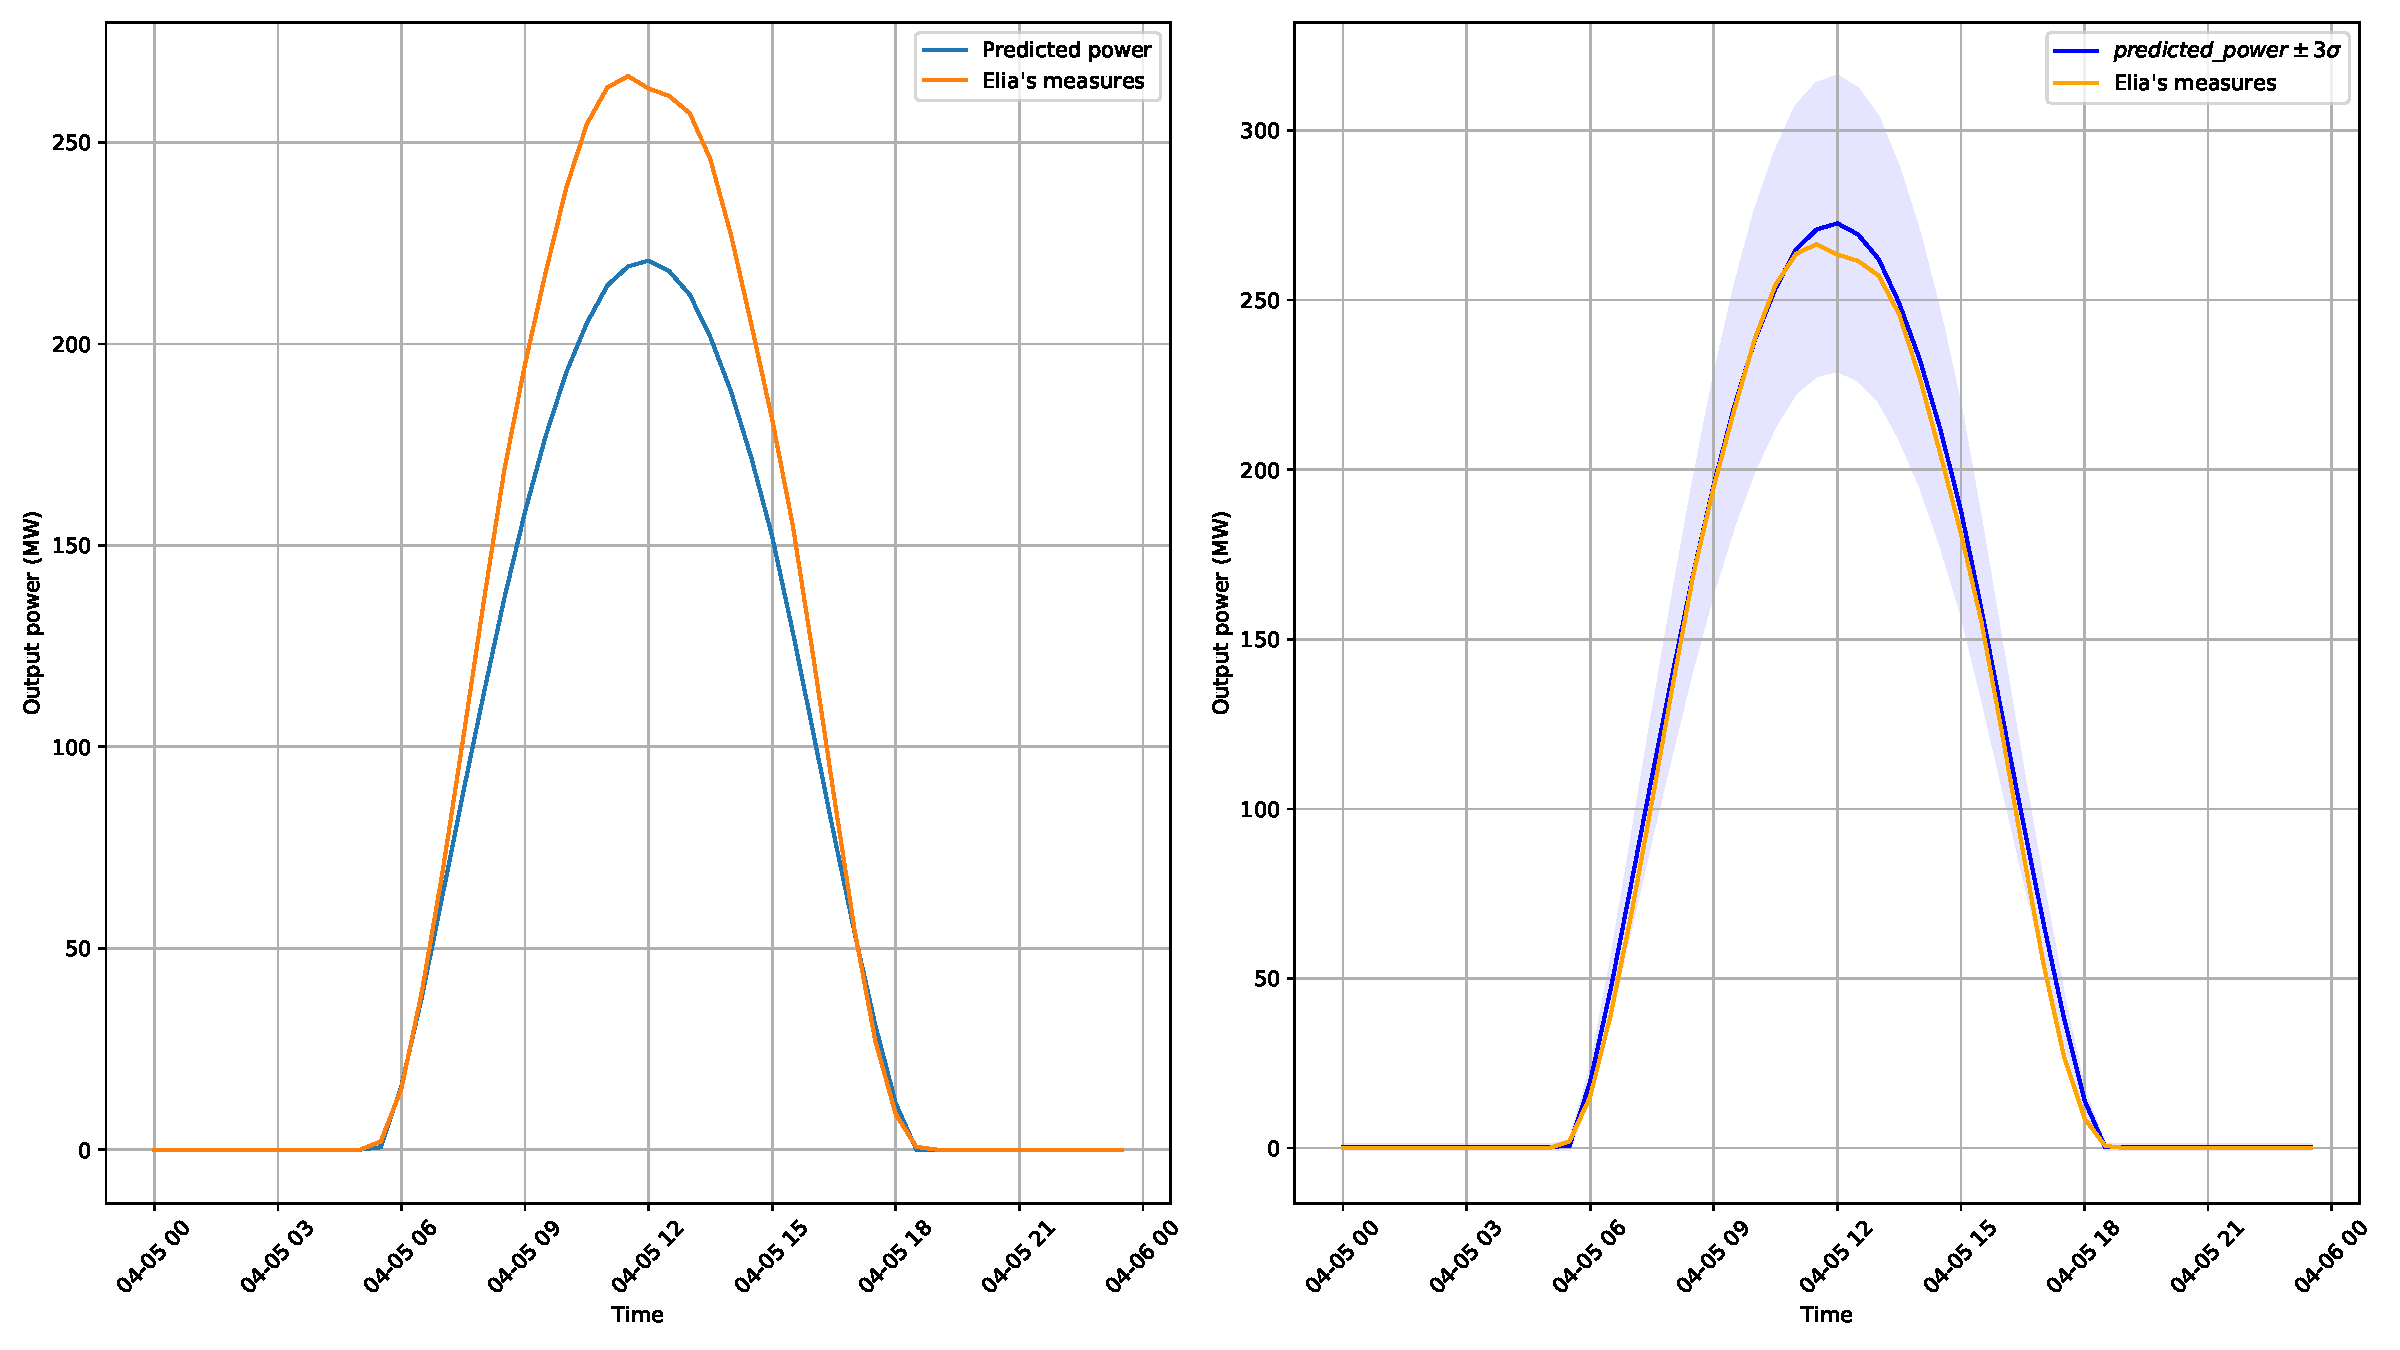
\includegraphics[width=\textwidth]{resources/pdf/comparison_naive_posterior_29-03-2020.pdf}
    \noskipcaption{Comparison between the naive predictive model and the posterior predictive model (April 5\up{th}).}
    \label{fig:naive_posterior_5_april}
\end{figure}
\begin{figure}[H]
    \centering
    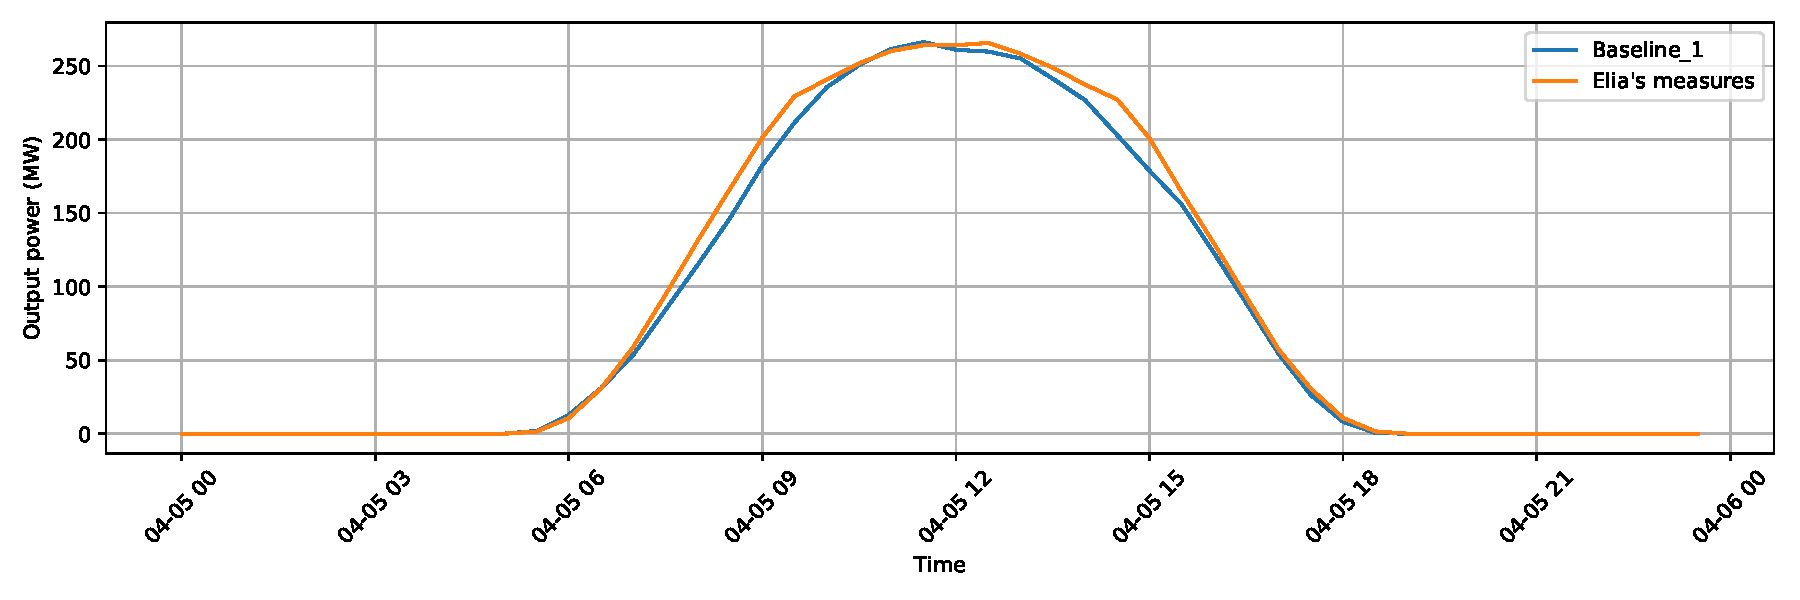
\includegraphics[width=\textwidth]{resources/pdf/baseline_1_29-03-2020.pdf}
    \noskipcaption{Comparison between the first baseline ($D-1$) and Elia's measures (April 5\up{th}).}
    \label{fig:base_1_elia_5_april}
\end{figure}
\begin{figure}[H]
    \centering
    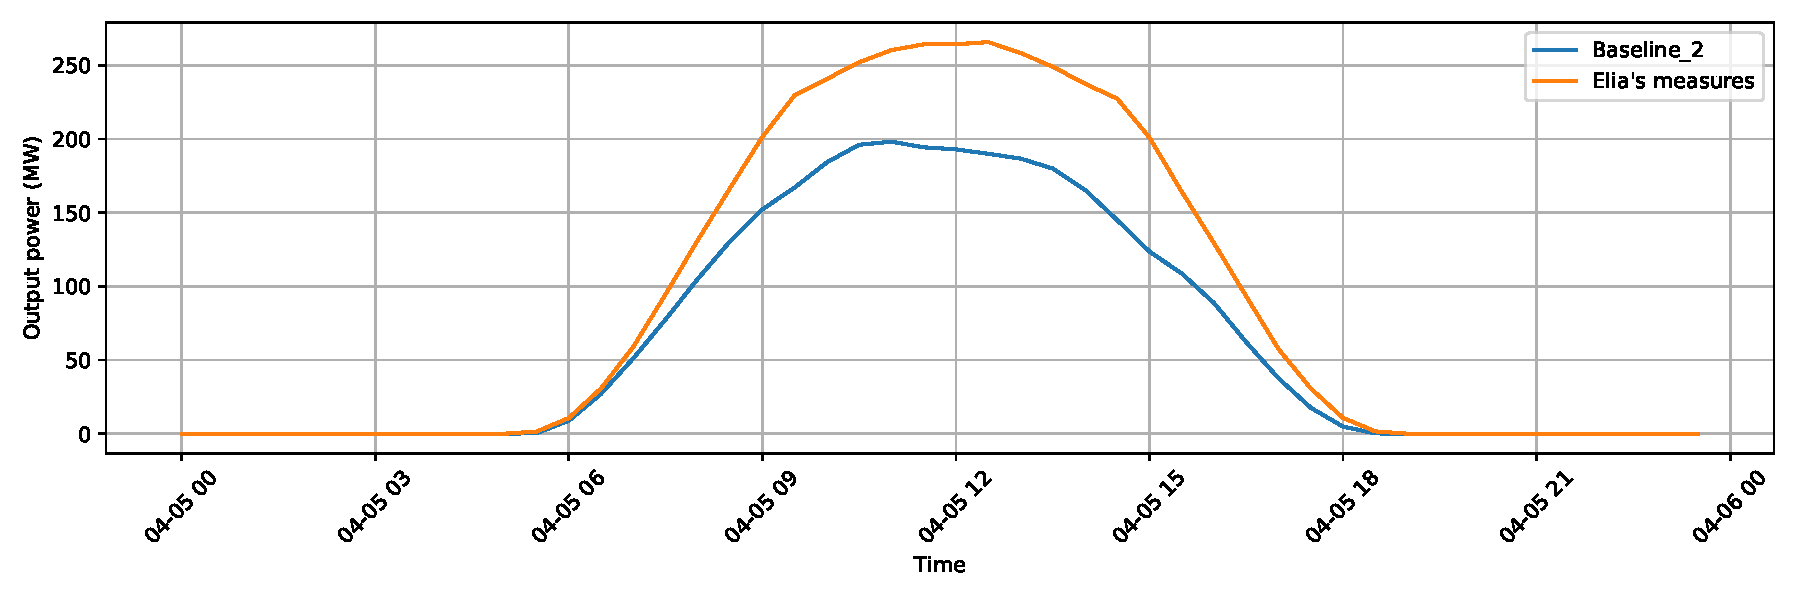
\includegraphics[width=\textwidth]{resources/pdf/baseline_2_29-03-2020.pdf}
    \noskipcaption{Comparison between the second baseline (average) and Elia's measures (April 5th).}
    \label{fig:base_2_elia_5_april}
\end{figure}
Situations where the baseline models perform slightly better than the posterior model correspond to, among other, situations like April 3\up{rd}, as can be seen on Figure \ref{fig:naive_posterior_3_april}, \ref{fig:base_1_elia_3_april} and \ref{fig:base_2_elia_3_april}.

\begin{figure}[H]
    \centering
    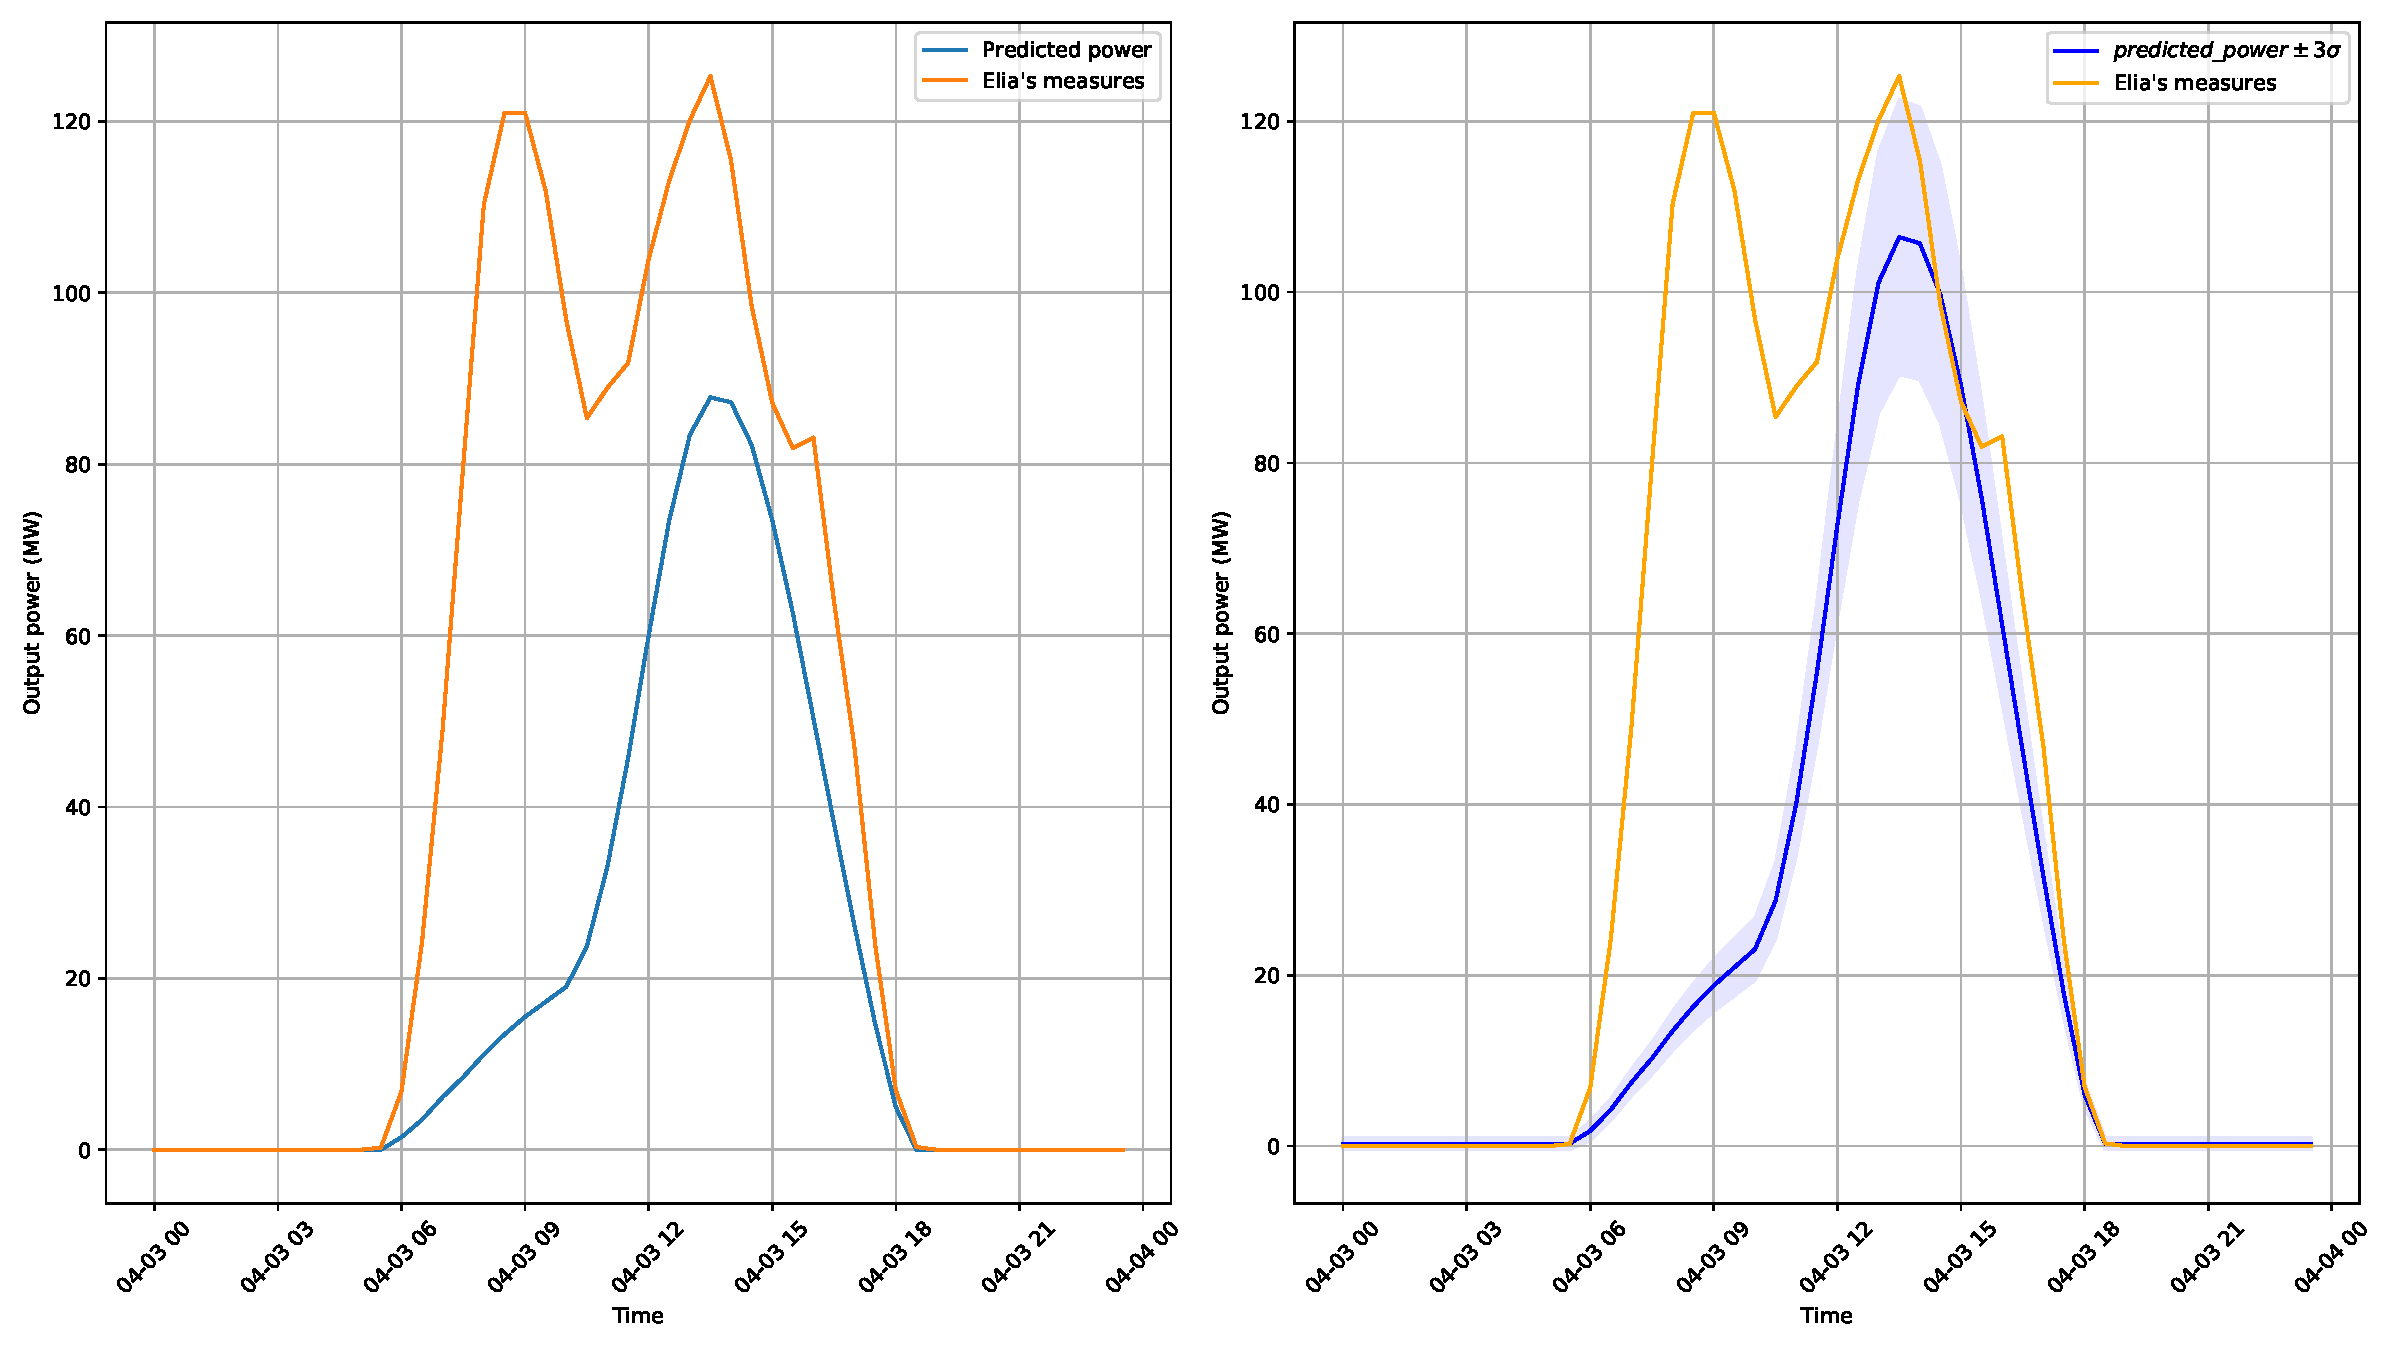
\includegraphics[width=\textwidth]{resources/pdf/comparison_naive_posterior_27-03-2020.pdf}
    \noskipcaption{Comparison between the naive predictive model and the posterior predictive model (April 3rd).}
    \label{fig:naive_posterior_3_april}
\end{figure}
\begin{figure}[H]
    \centering
    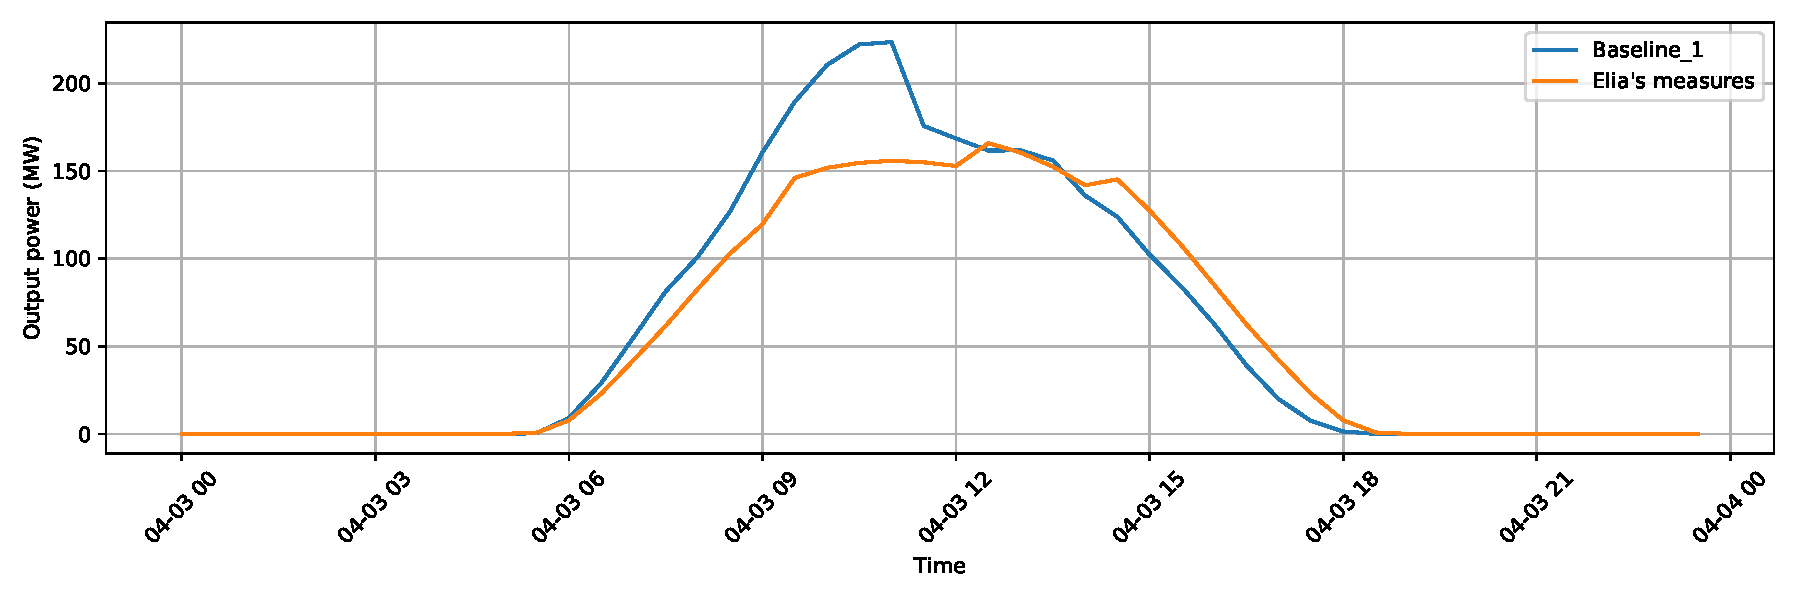
\includegraphics[width=\textwidth]{resources/pdf/baseline_1_27-03-2020.pdf}
    \noskipcaption{Comparison between the first baseline ($D-1$) and Elia's measures (April 3rd).}
    \label{fig:base_1_elia_3_april}
\end{figure}
\begin{figure}[H]
    \centering
    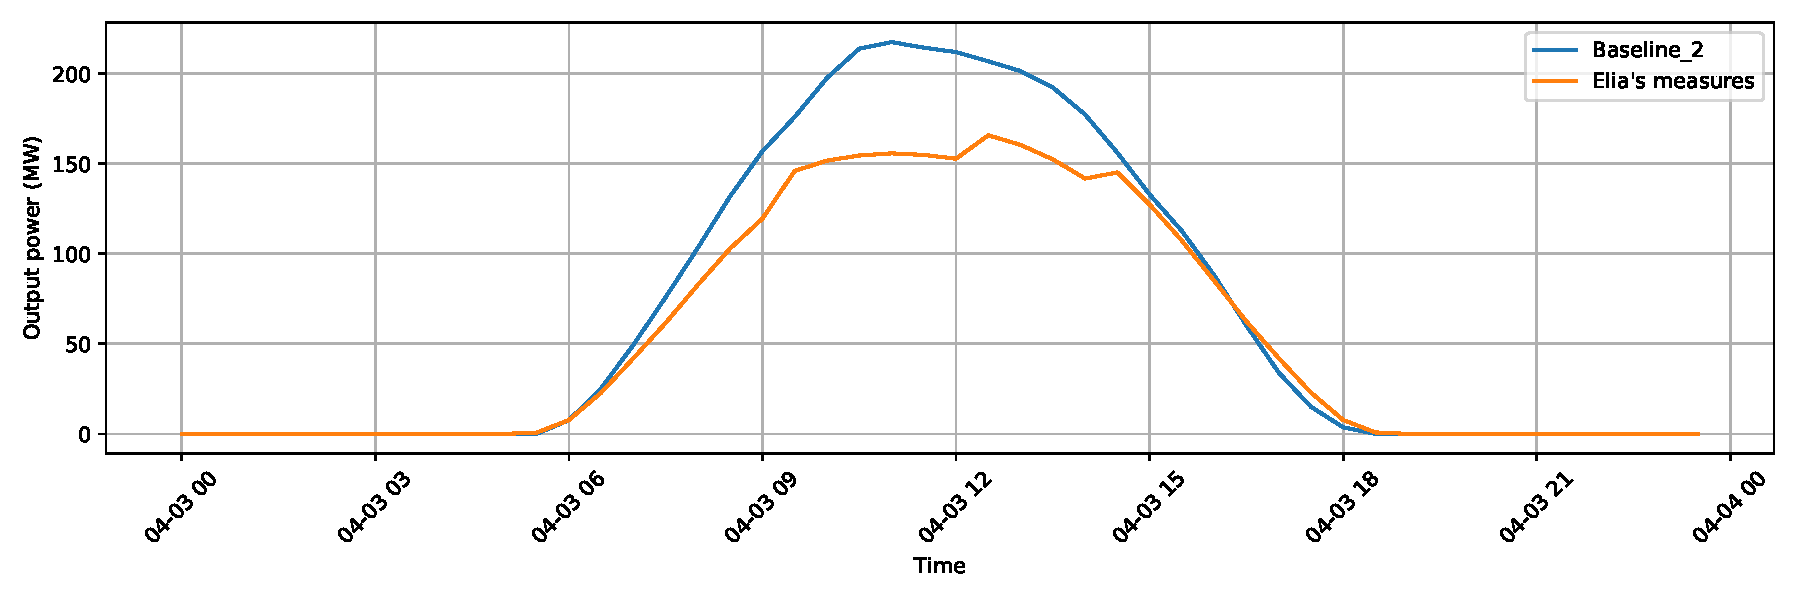
\includegraphics[width=\textwidth]{resources/pdf/baseline_2_27-03-2020.pdf}
    \noskipcaption{Comparison between the second baseline (average) and Elia's measures (April 3rd).}
    \label{fig:base_2_elia_3_april}
\end{figure}

We thus see that introducing irradiance forecast measures yields less precise models than those previously obtained, yet still reasonable. We can compare this with what we would have obtained for April 3\up{rd} using the measured irradiance instead of the forecast. The resulting posterior model can be seen on Figure \ref{fig:naive_post_meas}.
\begin{figure}[H]
    \centering
    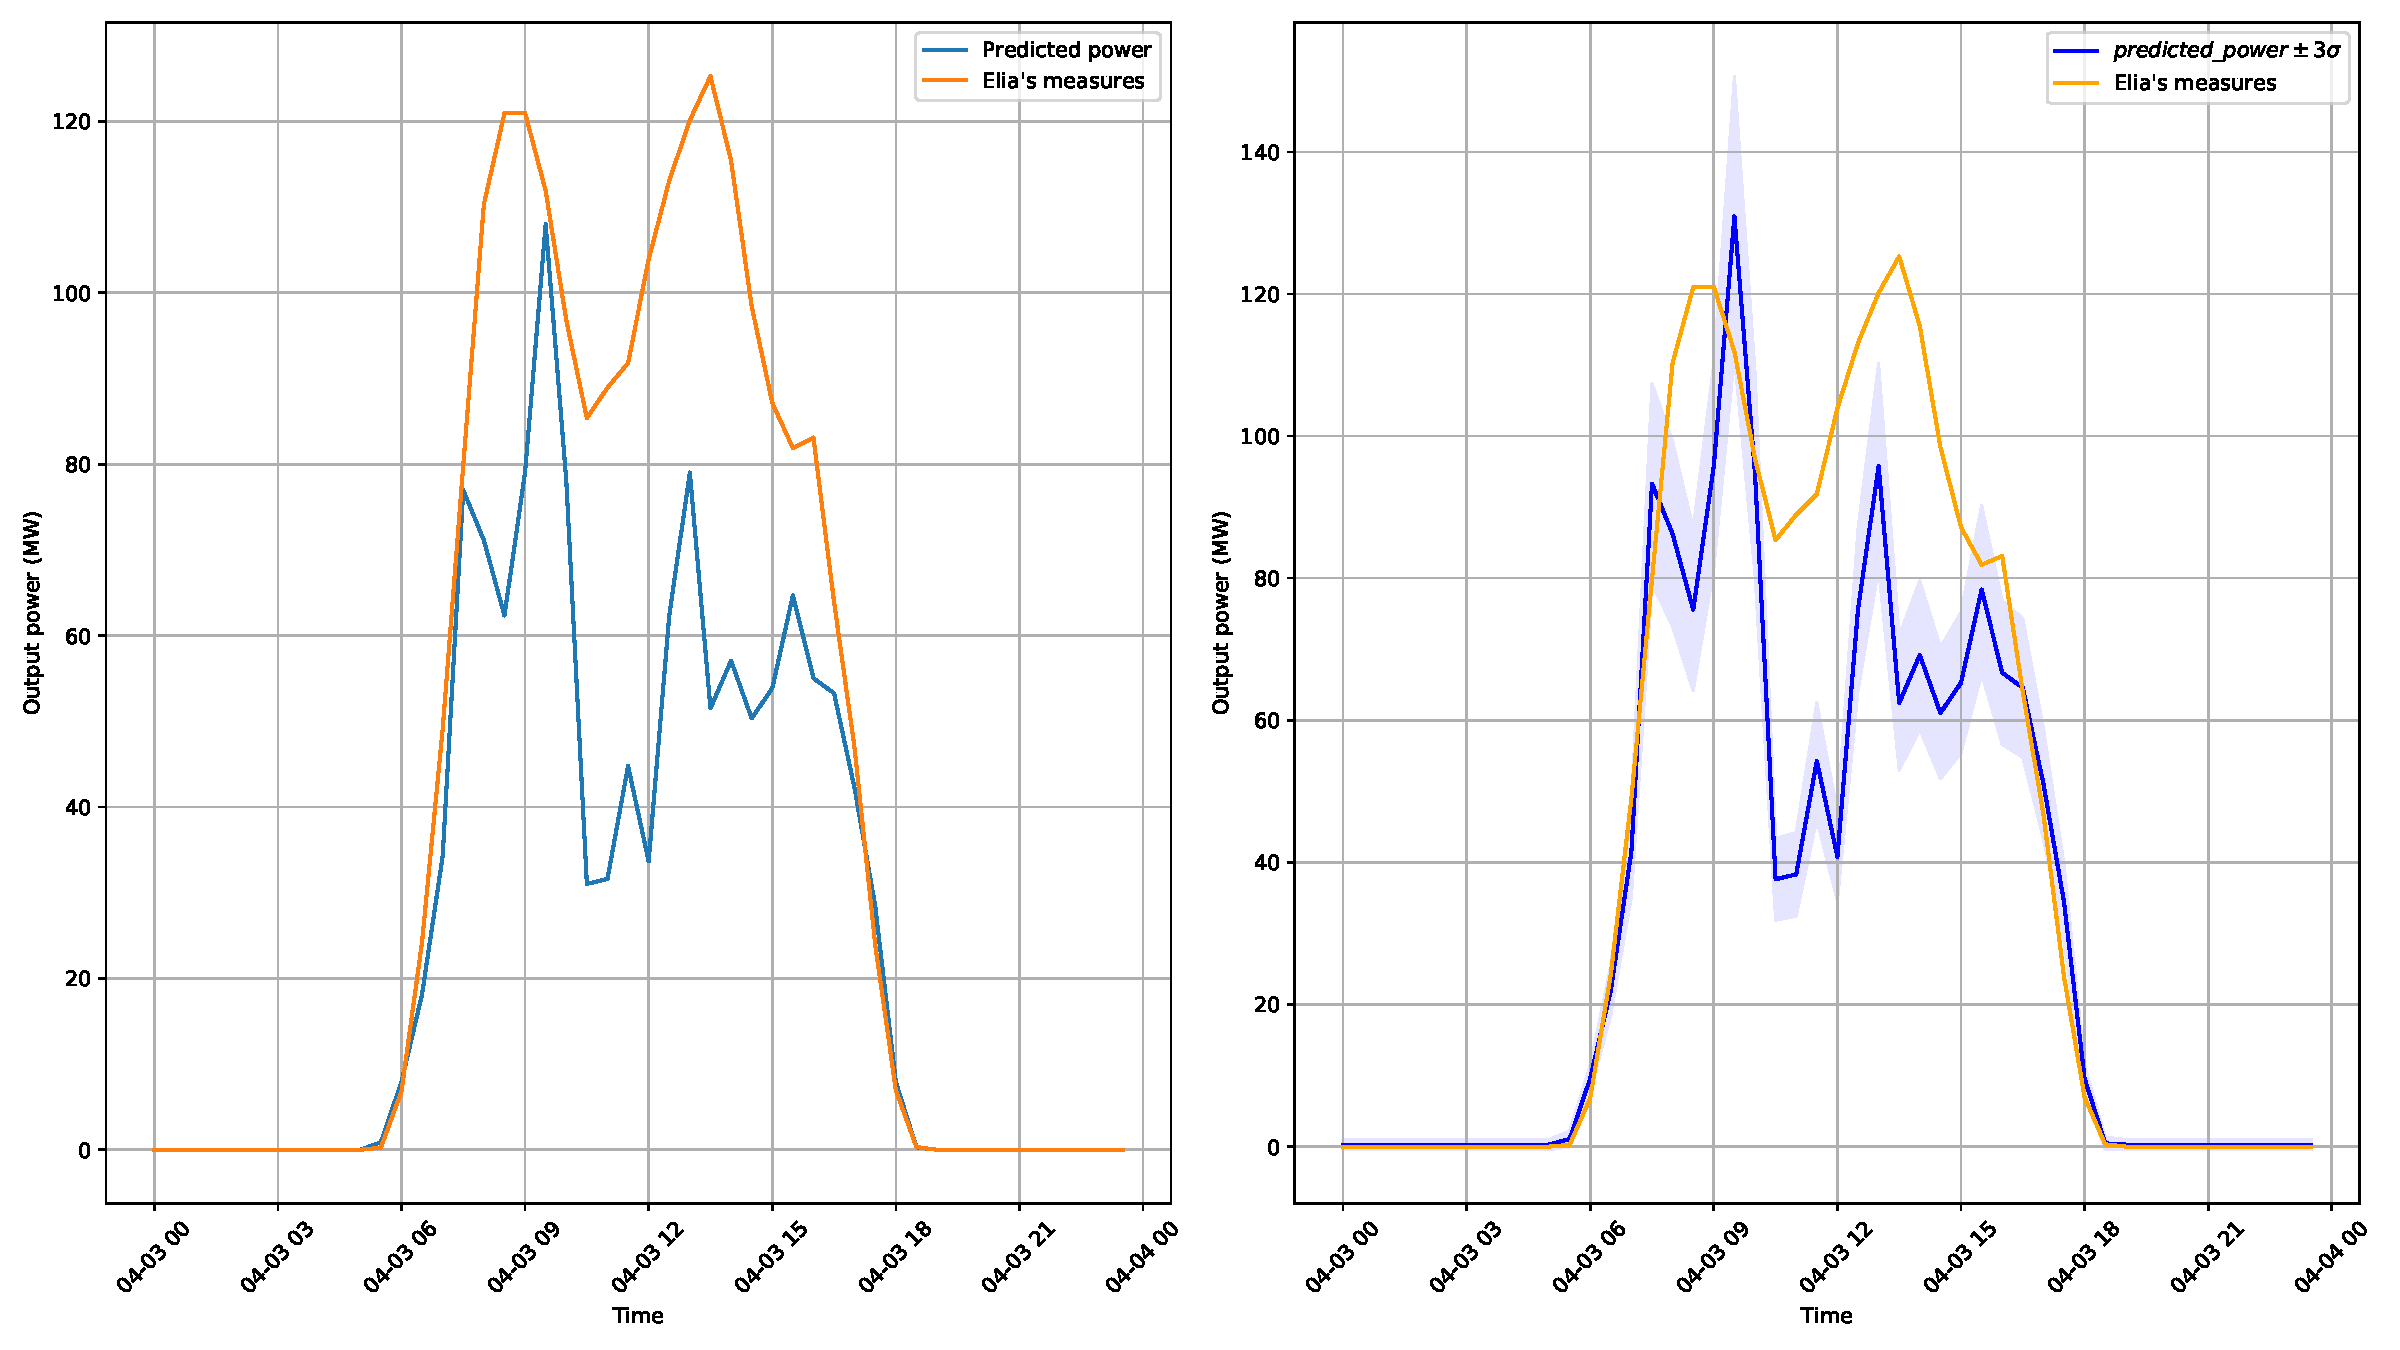
\includegraphics[width=\textwidth]{resources/pdf/comparison_naive_posterior_27-03-2020_meas.pdf}
    \noskipcaption{Comparison between the naive predictive model and the posterior predictive model (April 3\up{rd}) using the measurements.}
    \label{fig:naive_post_meas}
\end{figure}
From this, we can deduce that we would very likely have obtained a reduced MSE than with the forecast irradiance.

\subsection{Combining the panel enumerator and the solar model}
Finally, we took a first shot at combining the output of our panel enumerator with our initial model. However, since it should take quite more time to process all satellite images for the province of Liège, we have only computed data for the city of Liège.

For each panel installation, we have its corresponding latitude and longitude, its area as well as its surface azimuth. From there, it is straightforward to compute the output power of each installation, assuming a fixed tilt and a fixed efficiency $\eta$.

Since it only corresponds to the power produced in Liège, we cannot compare this series with Elia's measures. Hence, on Figure \ref{fig:solar_liege}, we decided to only represent the produced power for a period ranging from April 3\up{rd} to April 9\up{th}, using the irradiance forecast. We can then visually compare with Figure \ref{fig:prior_model} to see if the curves look similar.
\begin{figure}[H]
    \centering
    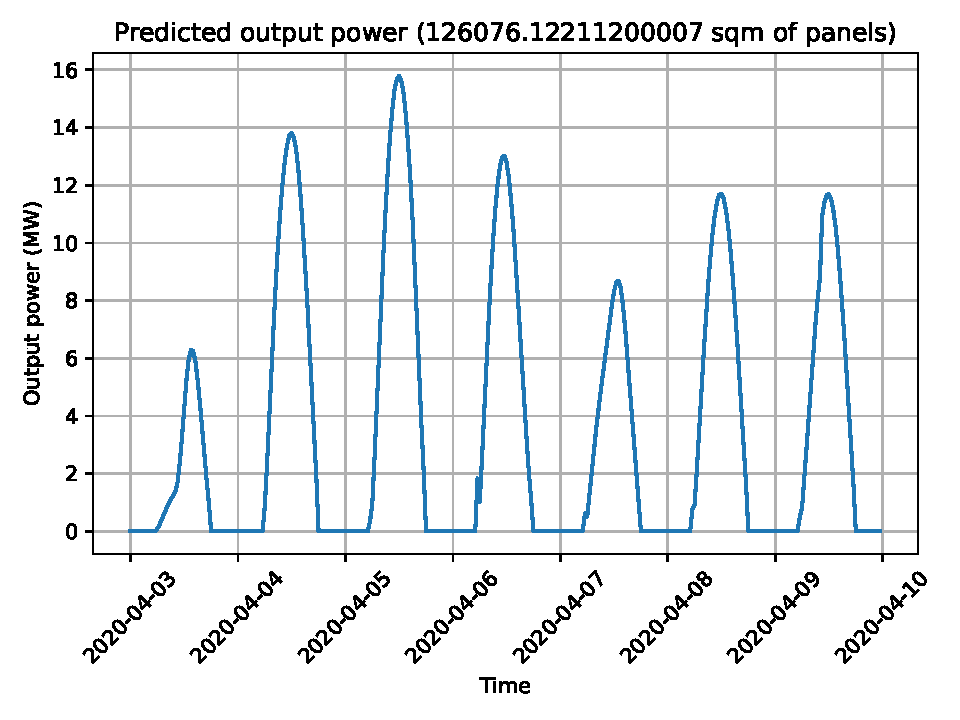
\includegraphics[width=0.8\textwidth]{resources/pdf/solar_liege.pdf}
    \noskipcaption{Predicted production in the city of Liège (using irradiance forecasts).}
    \label{fig:solar_liege}
\end{figure}
As we could already observe before, the obtained curves totally depend on the forecast irradiance curves, and they seem relatively good with respect to the curves measured by Elia. Nevertheless, the order of magnitude will depend on the output of our panel enumerator. Hence, we cannot really draw any conclusion right now since we only have data at the city scale.

\subsection{Next objectives}
For the final review, we will conduct these tests on a large part of April 2020 to get quite reliable error metrics estimates using irradiance forecasts.

Finally, we would also like to have processed as many satellite images as possible to estimate the area of photovoltaic panels in the province of Liège. This way, we could have another model for predicting the photovoltaic production at a provincial scale, and we will also then be able to compare to Elia's measures.

\newpage

\section{Photovoltaic panels enumeration}

The objectives of this review were pretty narrow : 

\begin{enumerate}[noitemsep]
    \item Apply our model to our initial problem, \emph{i.e.} the enumeration of panels in Liège.
    \item Evaluate more precisely the precision of our (U-Net) model using the \emph{average precision} metric.
\end{enumerate}

\subsection{WalOnMap}

To apply our model to the \emph{WalOnMap} \cite{walonmap} images, we first have to retrieve those images. Since the number of images is absolutely humongous (nearly \num{e6} for the province of Liège), it is not acceptable to store them. Therefore, we decided to implement an on-line method.

As we said in a previous review, these images are organized under the \emph{Web Map Tiles Service} standard \cite{maso2010opengis}. Therefore, we used the \texttt{owslib} package to request the tiles iteratively and release them directly after applying our model.

Obviously, we didn't want to save the produced masks on disk either. We chose to store them as polygons under the VGG Image Annotator \cite{dutta2019via} format. Most importantly, this format allows us to visualize (and modify) these polygons easily thanks to the provided open source software.

\begin{figure}[H]
    \centering
    \begin{subfigure}{0.49\textwidth}
        \centering
        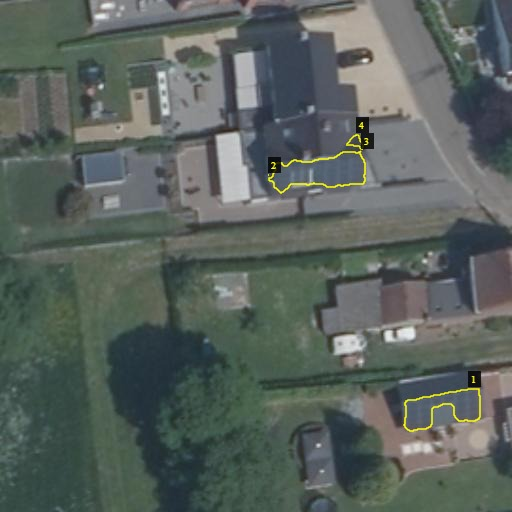
\includegraphics[width=0.8\textwidth]{resources/jpg/609089_533186.jpg}
        \vspace{0.5em}
    \end{subfigure}
    \begin{subfigure}{0.49\textwidth}
        \centering
        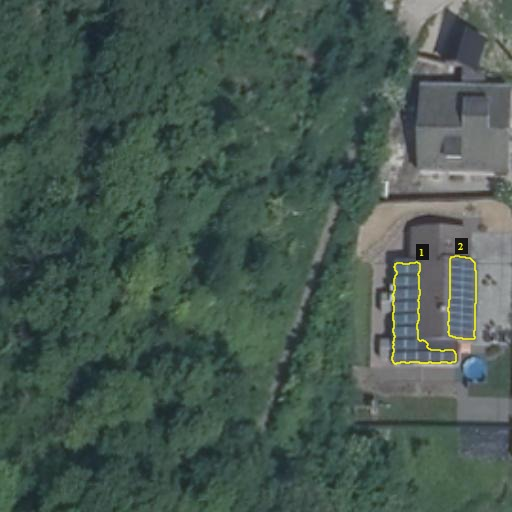
\includegraphics[width=0.8\textwidth]{resources/jpg/609089_533204.jpg}
        \vspace{0.5em}
    \end{subfigure}
    \begin{subfigure}{0.49\textwidth}
        \centering
        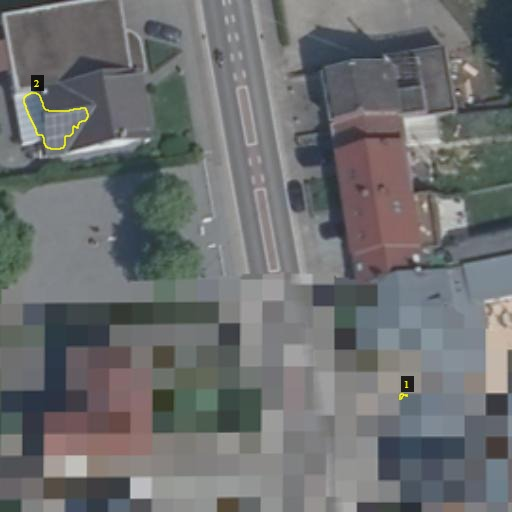
\includegraphics[width=0.8\textwidth]{resources/jpg/609090_533187.jpg}
    \end{subfigure}
    \begin{subfigure}{0.49\textwidth}
        \centering
        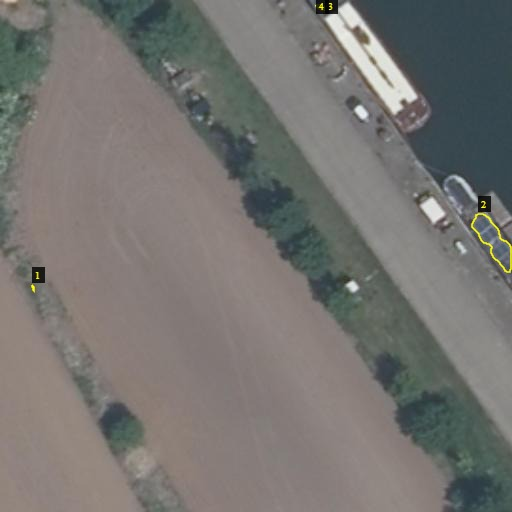
\includegraphics[width=0.8\textwidth]{resources/jpg/609090_533191.jpg}
    \end{subfigure}
    \noskipcaption{VGG Image Annotator polygons highlighting sample.}
    \label{fig:vgg_image_annotator}
\end{figure}

\begin{note}
We also have modified some of our previous implementations to better integrate this format to the framework.
\end{note}

\subsubsection{Applying the model}

The first time we applied the model, the performance\footnote{We retrieved the predictions and analyzed them subjectively.} were terrible : the predictions were basically random. We taught it was due to the blurriness of the WalOnMap images compared to the ones of California. Therefore, we pushed even further the data augmentation in training by adding blurring, smoothing and sharpening transformations.

This increased the performance on the Californian validation set (cf. section \ref{sec:average_precision}) but, unfortunately, it didn't help for the WalOnMap images. Then we realized that the scales of the two datasets were different. One pixel in Wallonia was about \SI{30}{\meter} where one pixel in California was about \SI{14}{\meter}. Therefore, we decided to upscale the images of California\footnote{We could have also down-scaled the images of Wallonia but that would have meant losing information.} by a factor \num{2}.

The performances improved dramatically, as most panels were now detected. Unfortunately, a lot of shadows\footnote{This is probably due to the fact that there are very little shadows in the Californian dataset as most pictures were taken at noon.} or dark roofs were also detected as panels.

To evaluate the actual performances of the model, we annotated by hand (using VIA) more than 600 WalOnMap images.

\begin{figure}[h]
    \centering
    \vspace{-0.5em}
    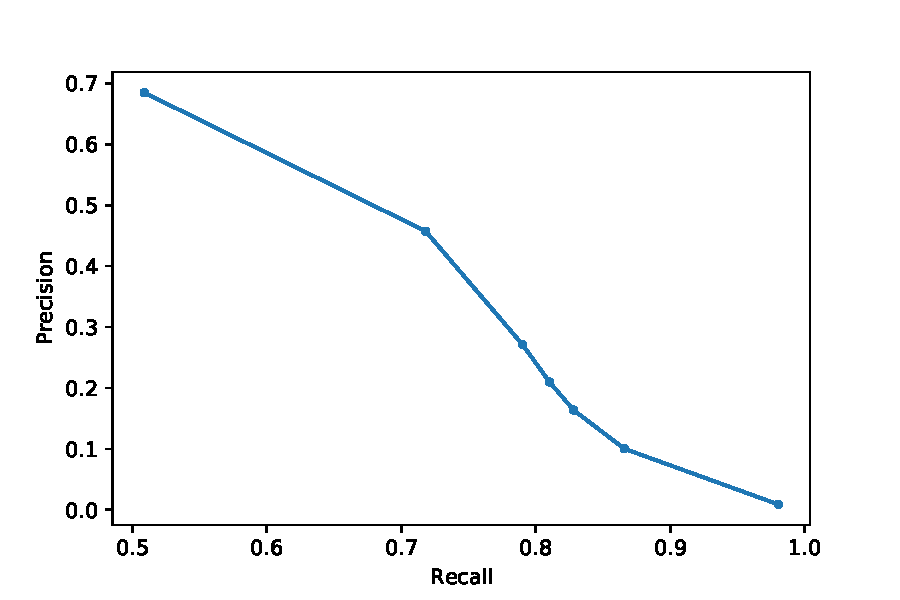
\includegraphics[width=0.8\textwidth]{resources/pdf/precision_recall_before.pdf}
    \caption{Precision-Recall curve of U-Net before fine tuning.}
    \label{fig:before_fine_tuning}
\end{figure}

As expected, our model had a respectable recall, but a very poor precision.

Therefore, we decided to train for a few (20) more epochs our model, but on a subset of the WalOnMap images we annotated by hand instead of the Californian ones. This technique is a special case of \emph{fine tuning}. As one can note by comparing Figures \ref{fig:before_fine_tuning} and \ref{fig:after_fine_tuning}, the performance boost was very significant !

\begin{figure}[h]
    \centering
    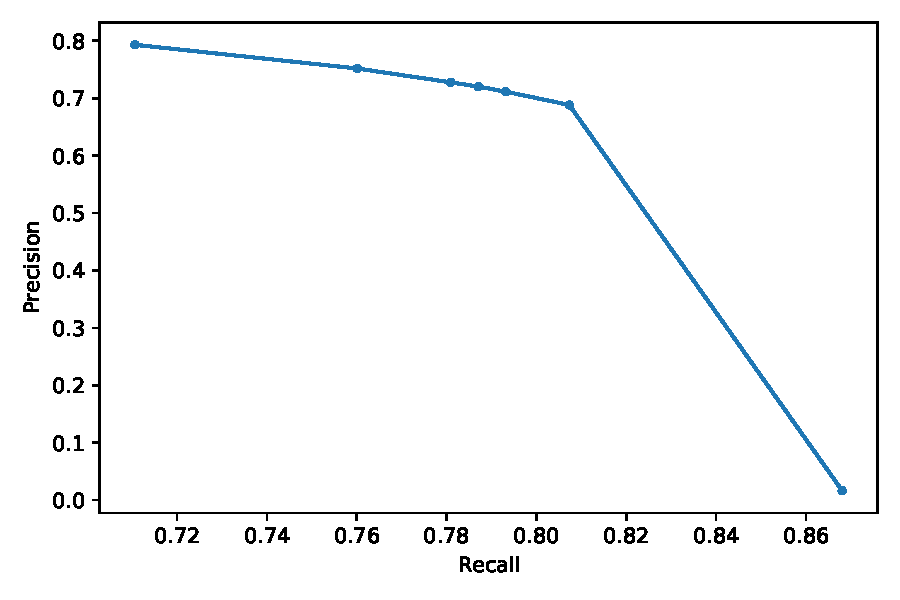
\includegraphics[width=0.75\textwidth]{resources/pdf/precision_recall_after.pdf}
    \caption{Precision-Recall curve of U-Net after fine tuning.}
    \label{fig:after_fine_tuning}
\end{figure}

\begin{note}
    Both curves were computed on the same WalOnMap subset never used for training. The polygons presented at Figure \ref{fig:vgg_image_annotator} were produced with our final model.
\end{note}

\subsubsection{Binding with the photovoltaic production model}

The last step was to bind our model outputs with the Photovoltaic production model. As explained in the corresponding section, the model requires the geographic position, the area and the azimuth angle for each solar installation.

Using some geospatial transformations and basic algebra, we managed to obtain a quite accurate measure of the position (1 to 2 meters off on average). Then, computing the area was straightforward as we already possessed the polygon vertices. However, computing the azimuth angle was another story.

Actually, we have no idea how to \emph{estimate} the azimuth based on the images. Therefore, we made hypothesis :

\begin{itemize}
    \item Most photovoltaic installations are greater than \SI{10}{\meter\squared};
    \item Most photovoltaic installations are rectangular shaped;
    \item The optimal orientation is south.
\end{itemize}

Based on these, we came up with the following procedure :

\begin{enumerate}
    \item If the polygon is too small (less than \SI{10}{\meter\squared}) we don't consider it, as it is probably noise.
    \item We compute the \emph{minimal area bounding rectangle} of the polygon.
    \item We compute the azimuth based on the rotation angle of this rectangle and optimizing the orientation towards south.
\end{enumerate}

All these measures are then saved in a ready-to-use \texttt{JSON} file.

\subsection{Average precision}\label{sec:average_precision}

In the last review, we presented the precision and recall of our model at a threshold of \num{0.5}. In the computer vision field, the Average Precision is often used to isolate these performance measures from any threshold.

\begin{figure}[h]
    \centering
    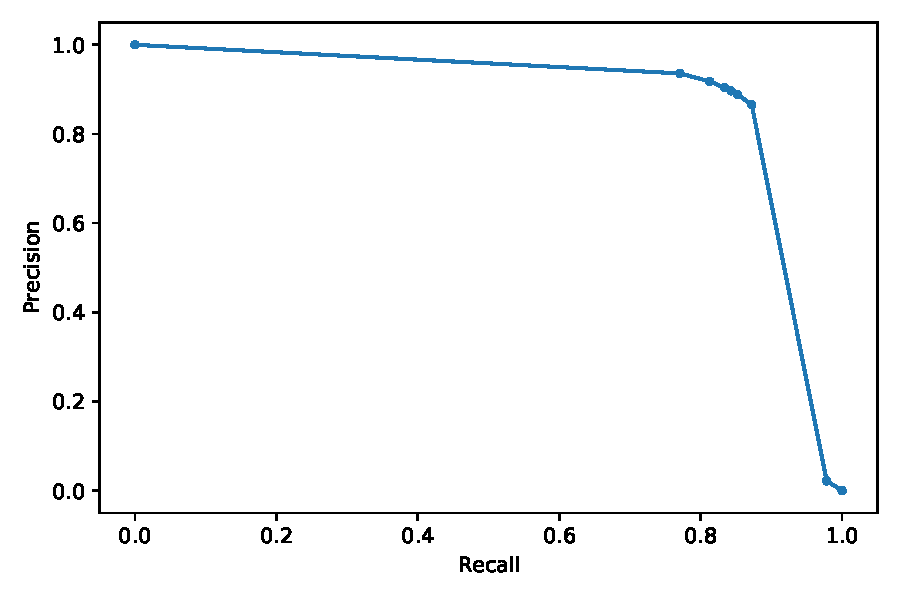
\includegraphics[width=0.75\textwidth]{resources/pdf/precision_recall.pdf}
    \caption{Precision-Recall curve of U-Net on the Californian validation set.}
    \label{fig:after_fine_tuning}
\end{figure}

The obtained average precision (the area under the curve) is \SI{88.6}{\percent} which is quite respectable.

\subsubsection{Training convergence}

\begin{figure}[H]
    \centering
    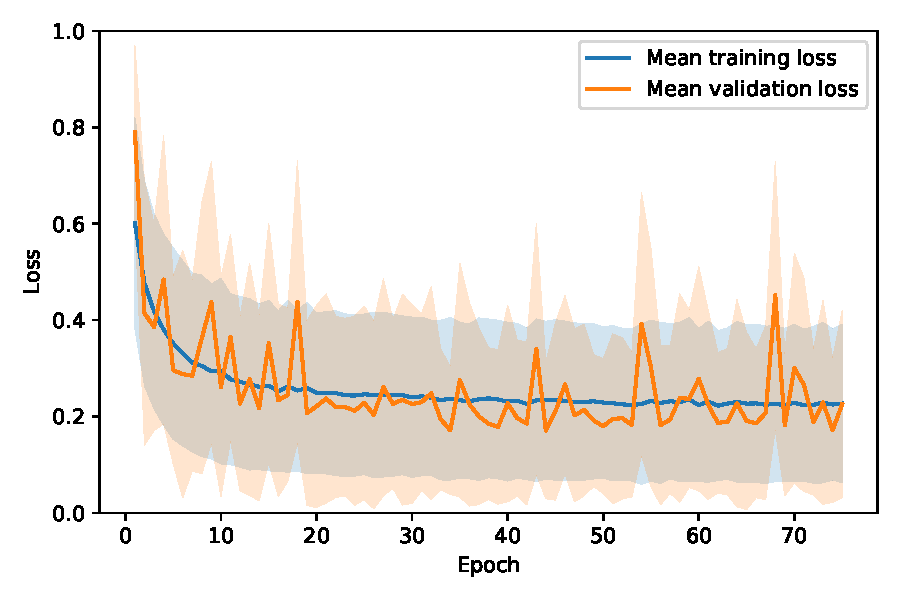
\includegraphics[width=0.75\textwidth]{resources/pdf/mean_loss.pdf}
    \noskipcaption{Mean dice losses with respect to the epochs.}
    \label{fig:mean_loss}
\end{figure}

\begin{figure}[H]
    \centering
    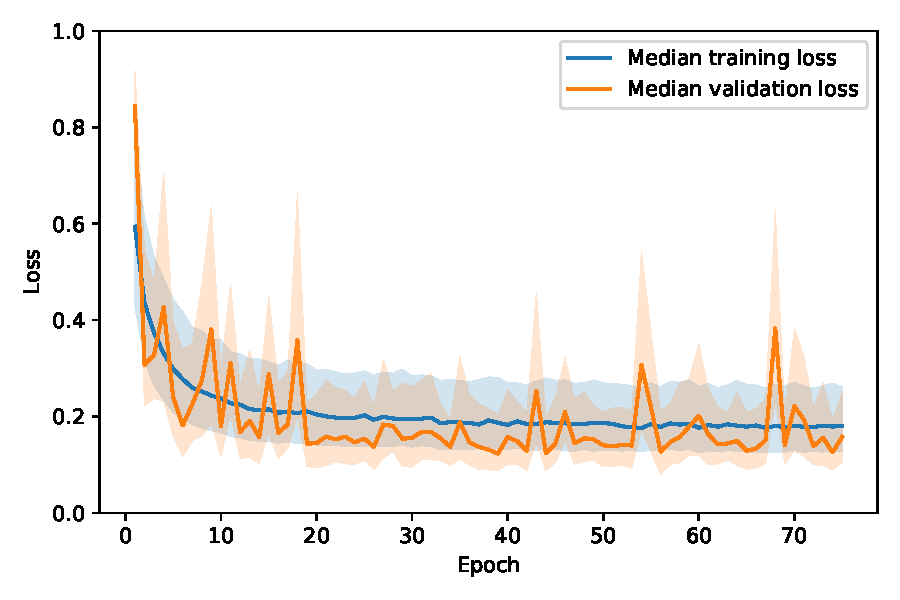
\includegraphics[width=0.75\textwidth]{resources/pdf/median_loss.pdf}
    \noskipcaption{Median dice losses with respect to the epochs.}
    \label{fig:median_loss}
\end{figure}

\begin{note}
    The Figures \ref{fig:mean_loss} and \ref{fig:median_loss} are given as-is and won't be analyzed here, as it is not within the scope of this project.
\end{note}

\subsection{Next objectives}

As said in the photovoltaic production section, we didn't have time to process the whole province, so we reduced the scope to the city of Liège. The next step is obviously to apply the model to all ($\pm$ \num{9e5}) tiles in the province. According to our estimations, it should take between 2 and 3 days.

Also, we still have to try other models, but we think it won't be part of this course final report but rather the Deep Learning report.

\newpage

\section{Wind Production}

With regard to the good results obtained by our statistical model (weather to power model), we have chosen to focus on this statistical approach and leave aside the physical model and its possible improvements. The idea of an hybrid model is thus discarded too.

Several things had to be done for this review: adding temporal variables to the model such as the total installed power, testing a last supervised learning method: the multilayer perceptron, and finally assessing the features importances. No feature selection has been performed yet, in order to compare the addition of the new variables and the multilayer perceptron with the best model of review 4 (Gradient Boosting on 15 7-dimensional weather measurements: 105 variables).

All metric scores are obtained using the protocol 2 of last review: random shuffling of the dataset, as it certainly yields a validation set with lower bias.

\subsection{Results of the addition of new variables}

Unfortunately, the addition of the following new variables has not helped the model performing better: 
\begin{itemize}
    \item Total power monitored by Elia
    \item Yearly total installed power in Wallonia
    \item One day before power measurements
\end{itemize}

The results can be found in table \ref{tab:new_variables_gb}, they are compared to the best model of last review (preferred for its better quantiles): Gradient Boosting on the 105 weather variables, but are also compared to the Extra trees on the 105 weather variables.

\begin{table}[H]
    \centering
    \begin{tabular}{|c|c|c|c|c|c|}
        \hline
        Protocol & Method & MAE & sMAE & MQL10 & MQL90 \\ \hline
        \multirow{2}{*}{With the new variables} & Extra Trees & 28.27 & 4.43\% & 53.42 & 56.33 \\ \cline{2-6}
         & Gradient Boosting & 30.98 & 4.27\% & 51.23 & 55.21 \\ \hline
        \multirow{2}{*}{Without the new variables} & Extra Trees & 28.13 & 4.03\% & 46.63 & 50.32 \\ \cline{2-6}
         & Gradient Boosting & 31.11 & 4.46\% & 48.32 & 47.91 \\ \hline
    \end{tabular}
    \caption{Effect of the new variables on the models' scores on validation set}
    \label{tab:new_variables_gb}
\end{table}

As this results are not convincing at all, it has been chosen not to keep these new variables.

\subsection{Results for the multilayer perceptron}

Several network structures have been tried, the results were as good as the Gradient Boosting methods, for example the best results obtained with a MLP with the following hidden layers: $1000, 1000, 300, 50$ are given in table \ref{tab:mlp}.

\begin{table}[]
    \centering
    \begin{tabular}{|c|c|c|}
        \hline 
        Method & MAE & sMAE \\ \hline
        MLP & 30.98 & 4.27\%  \\ \hline
    \end{tabular}
    \caption{Multilayer Perceptron scores on validation set}
    \label{tab:mlp}
\end{table}

This multilayer perceptron has not been extanded to quantile regression because it didn't give better results than the Gradient Boosting method, the latter being thus preferred.

\subsection{Alternative to improve the Gradient Boosting model}

As no model seemed to be able to perform better than what we have reached at last review, we tried to get more precise explanatory variables: weather measurements at each power plant instead of just the 15 locations hand pinned. We have thus started collected a new dataset of 68 7-dimensional weather measurements in order to replace our 105-variables dataset by a 476-variables dataset. The map of power plants of Wallonia and new weather measurements is on figure \ref{fig:wt_wallonia}.

\begin{figure}[H]
    \centering
    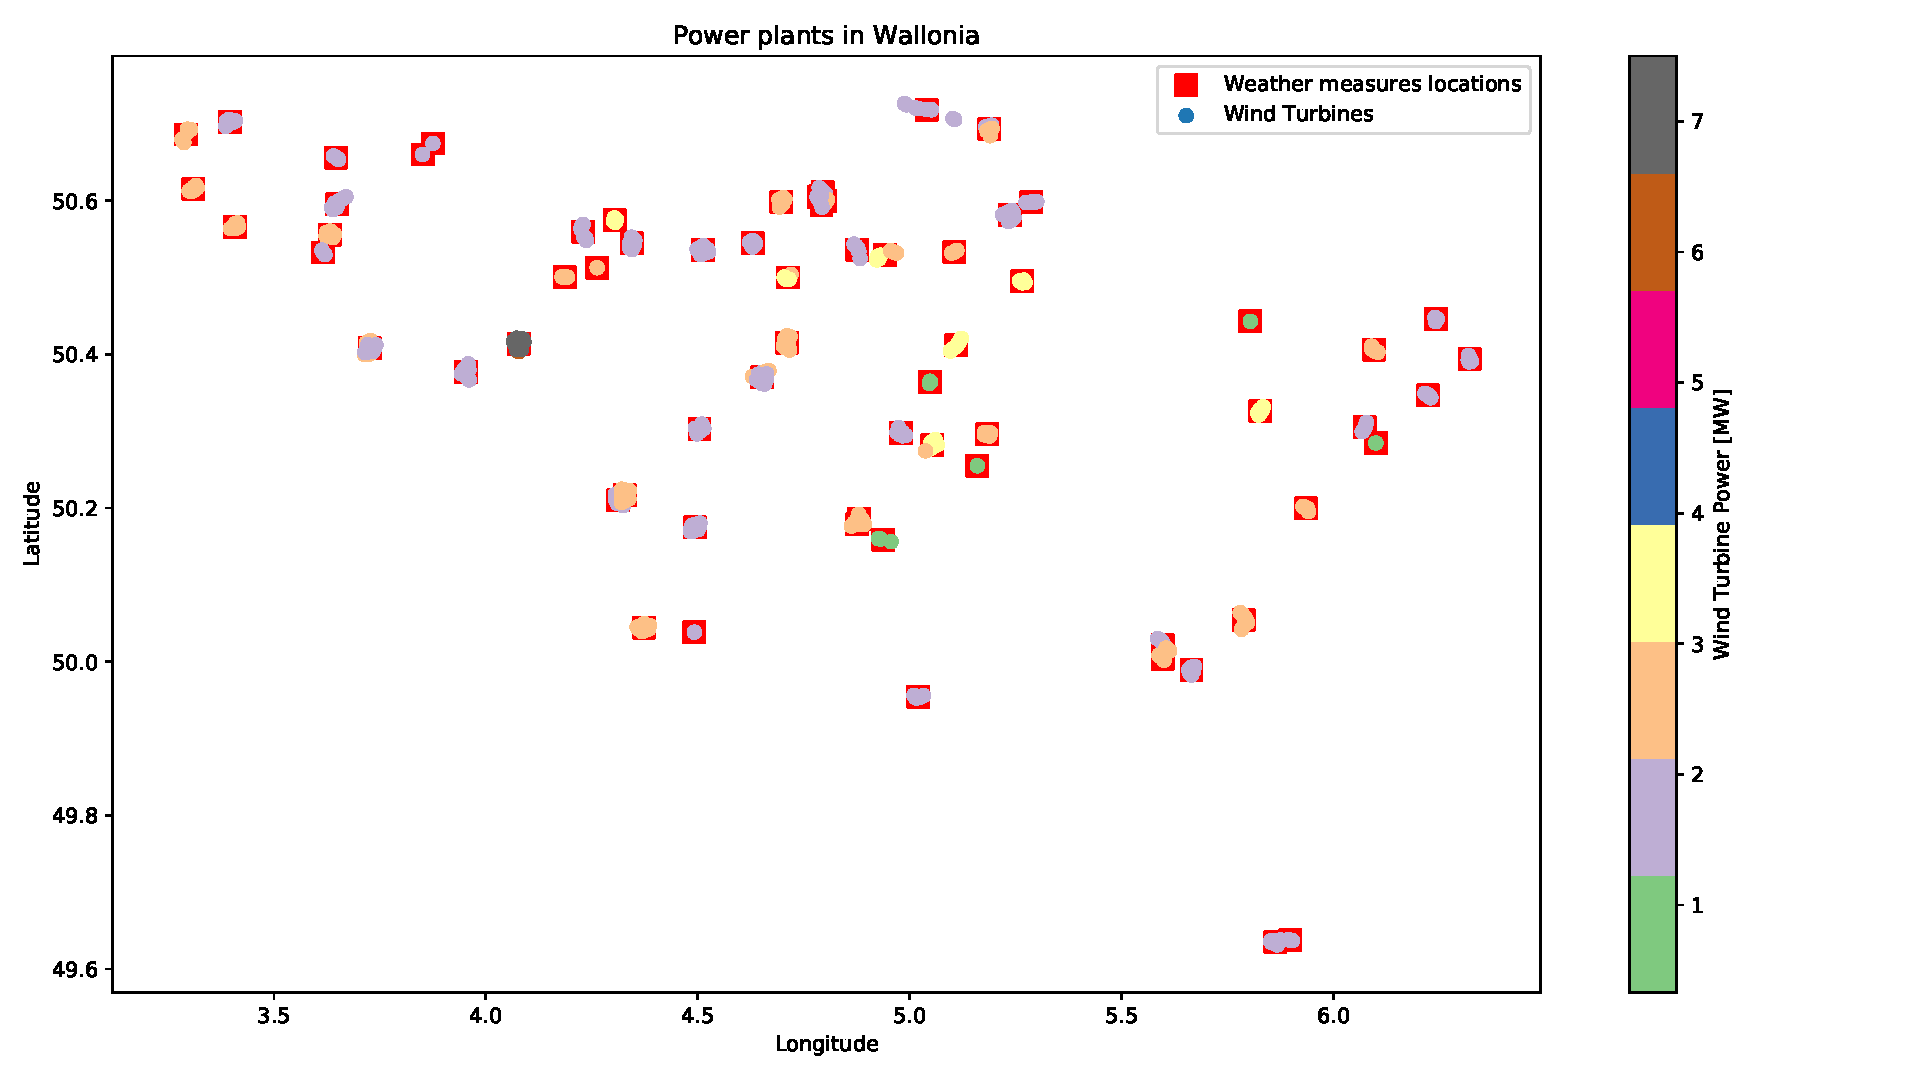
\includegraphics[width=\textwidth]{resources/pdf/power_plants.pdf}
    \caption{Wind turbines and weather measurements}
    \label{fig:wt_wallonia}
\end{figure}

As can be seen in table \ref{tab:wind68}, using these new variables with one 7-dimensional weather measurement per power plant instead of the 15 hand pinned weather measurements yielded slightly better results on the validation set.

\begin{table}[H]
    \centering
    \begin{tabular}{|c|c|c|c|c|}
        \hline
        Method & MAE & sMAE & MQL10 & MSL90 \\ \hline
        Gradient Boosting 15 & 31.11 & 4.46\% & 48.32 & 47.91 \\ \hline
        Gradient Boosting 68 & 28.46 & 3.92\% & 51.19 & 49.33 \\ \hline
    \end{tabular}
    \caption{Gradient Boosting with 68 weather measurements' scores on validation set}
    \label{tab:wind68}
\end{table}

\paragraph{Results on the test set}

The test set is composed of Day-Ahead Numerical Weather Prediction (DANWP), it means that the model is tested in real condition where we use the weather forecasts instead of the weather measurements. A test set has been built from March 19 for the 15-measurements model, and another test set has been built from April 5 for the 68-measurements model.

First, we can have a look at the results for the 15-measurements model from March 19 in figure \ref{fig:odaf15}. The MAE is 52.56 in this case on this period, which is to be compared with the MAE of 31.1 obtained by the same model on the validation set (weather measurements instead of DANWP). We can clearly see that the uncertainty on the weather forecast (MAE around \SI{2.4}{\meter\per{\second}} for the wind speed for example) deteriorates our results by less than 200\% in terms of MAE. This is better than what we expected, since we had conclude a worst case deterioration of 300\%.

\begin{figure}[H]
    \centering
    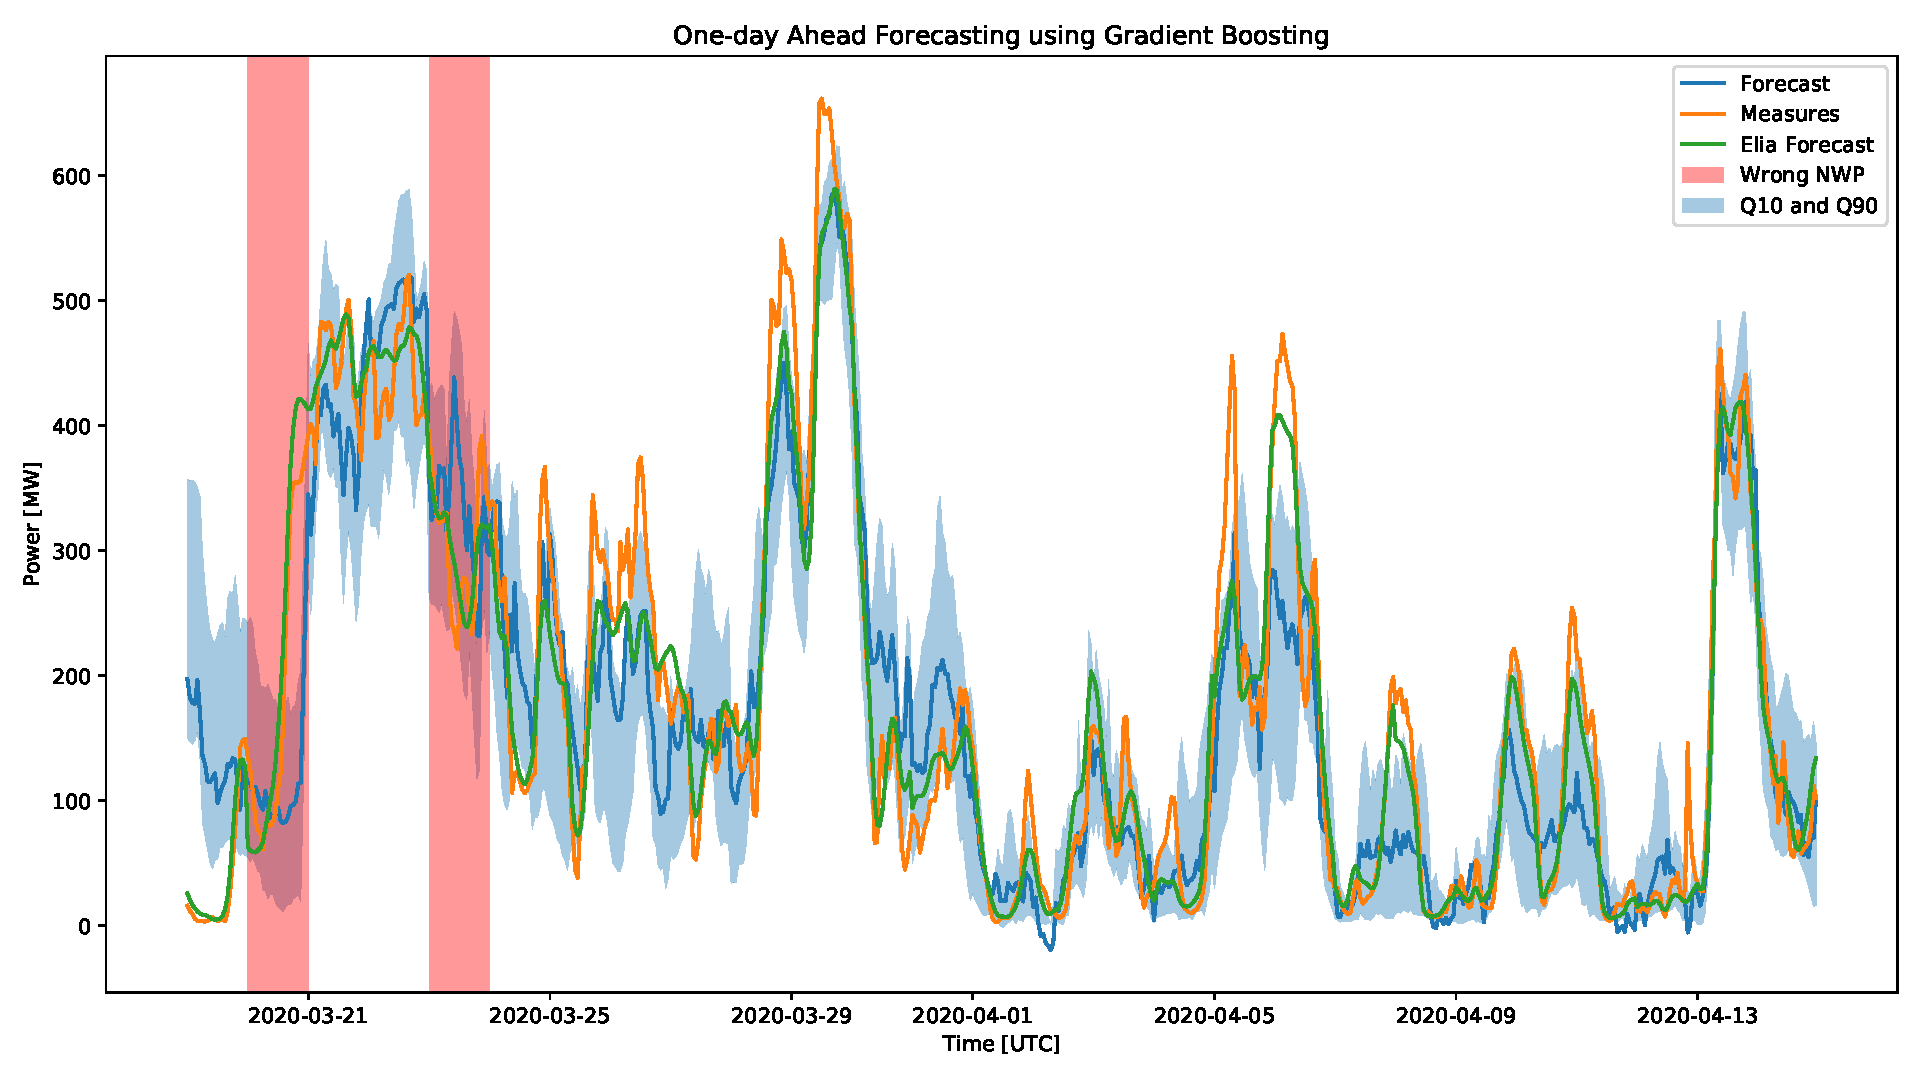
\includegraphics[width=\textwidth]{resources/pdf/odaf15.pdf}
    \caption{Day-Ahead Forecast using 15-measurements Gradient Boosting}
    \label{fig:odaf15}
\end{figure}

Then, we can compare the prediction from April 5 of the 15-measurements model and the 68-measurements model on figure \ref{fig:wind_test_april}. The MAE are respectively 45.42 and 40.72, but the test set is only 9.5 days long for now, and these results should be taken with care. The test set on 68 measurements is grown each day, and we will be able to present stronger conclusions for the next review.

\begin{figure}[H]
    \begin{subfigure}{1\textwidth}
        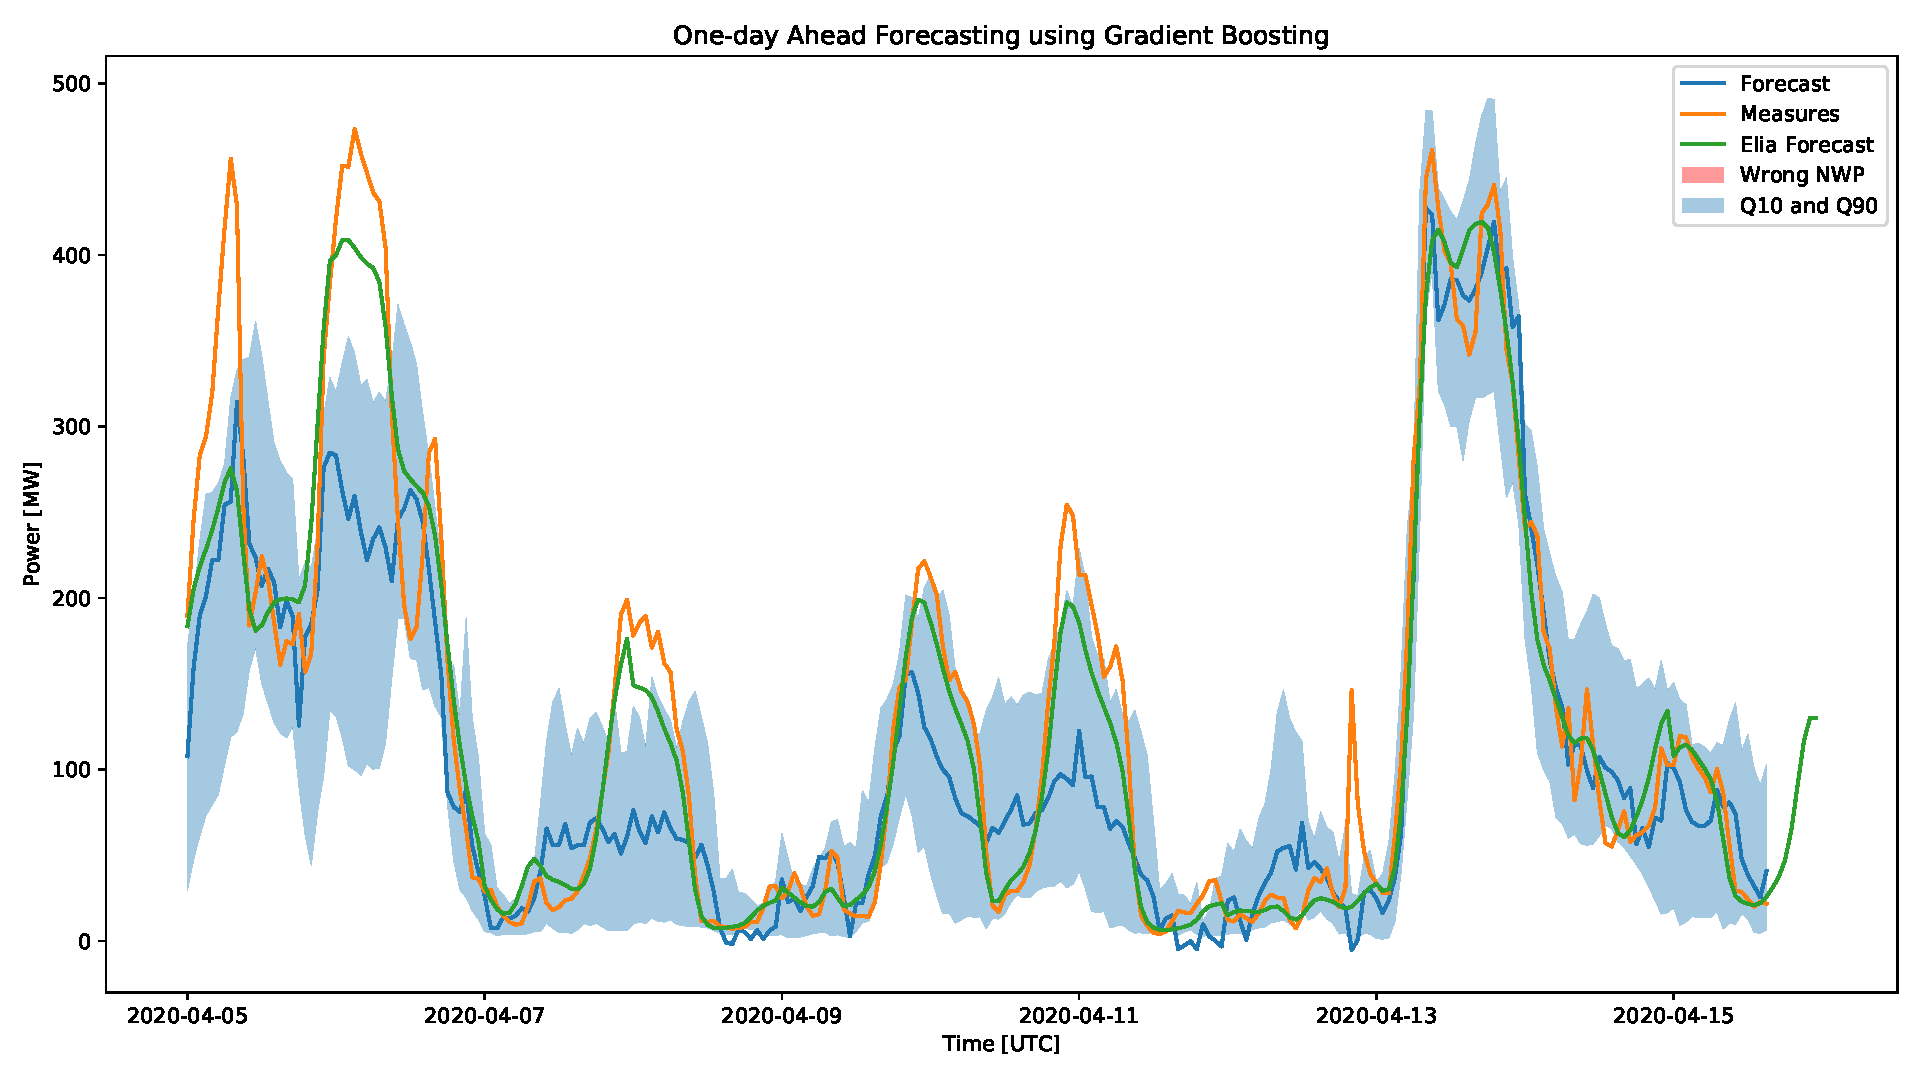
\includegraphics[width=\textwidth]{resources/pdf/odaf15_april.pdf}
        \caption{15-measurements Gradient Boosting}
    \end{subfigure}
    
    \vspace{1em}
    
    \begin{subfigure}{1\textwidth}
        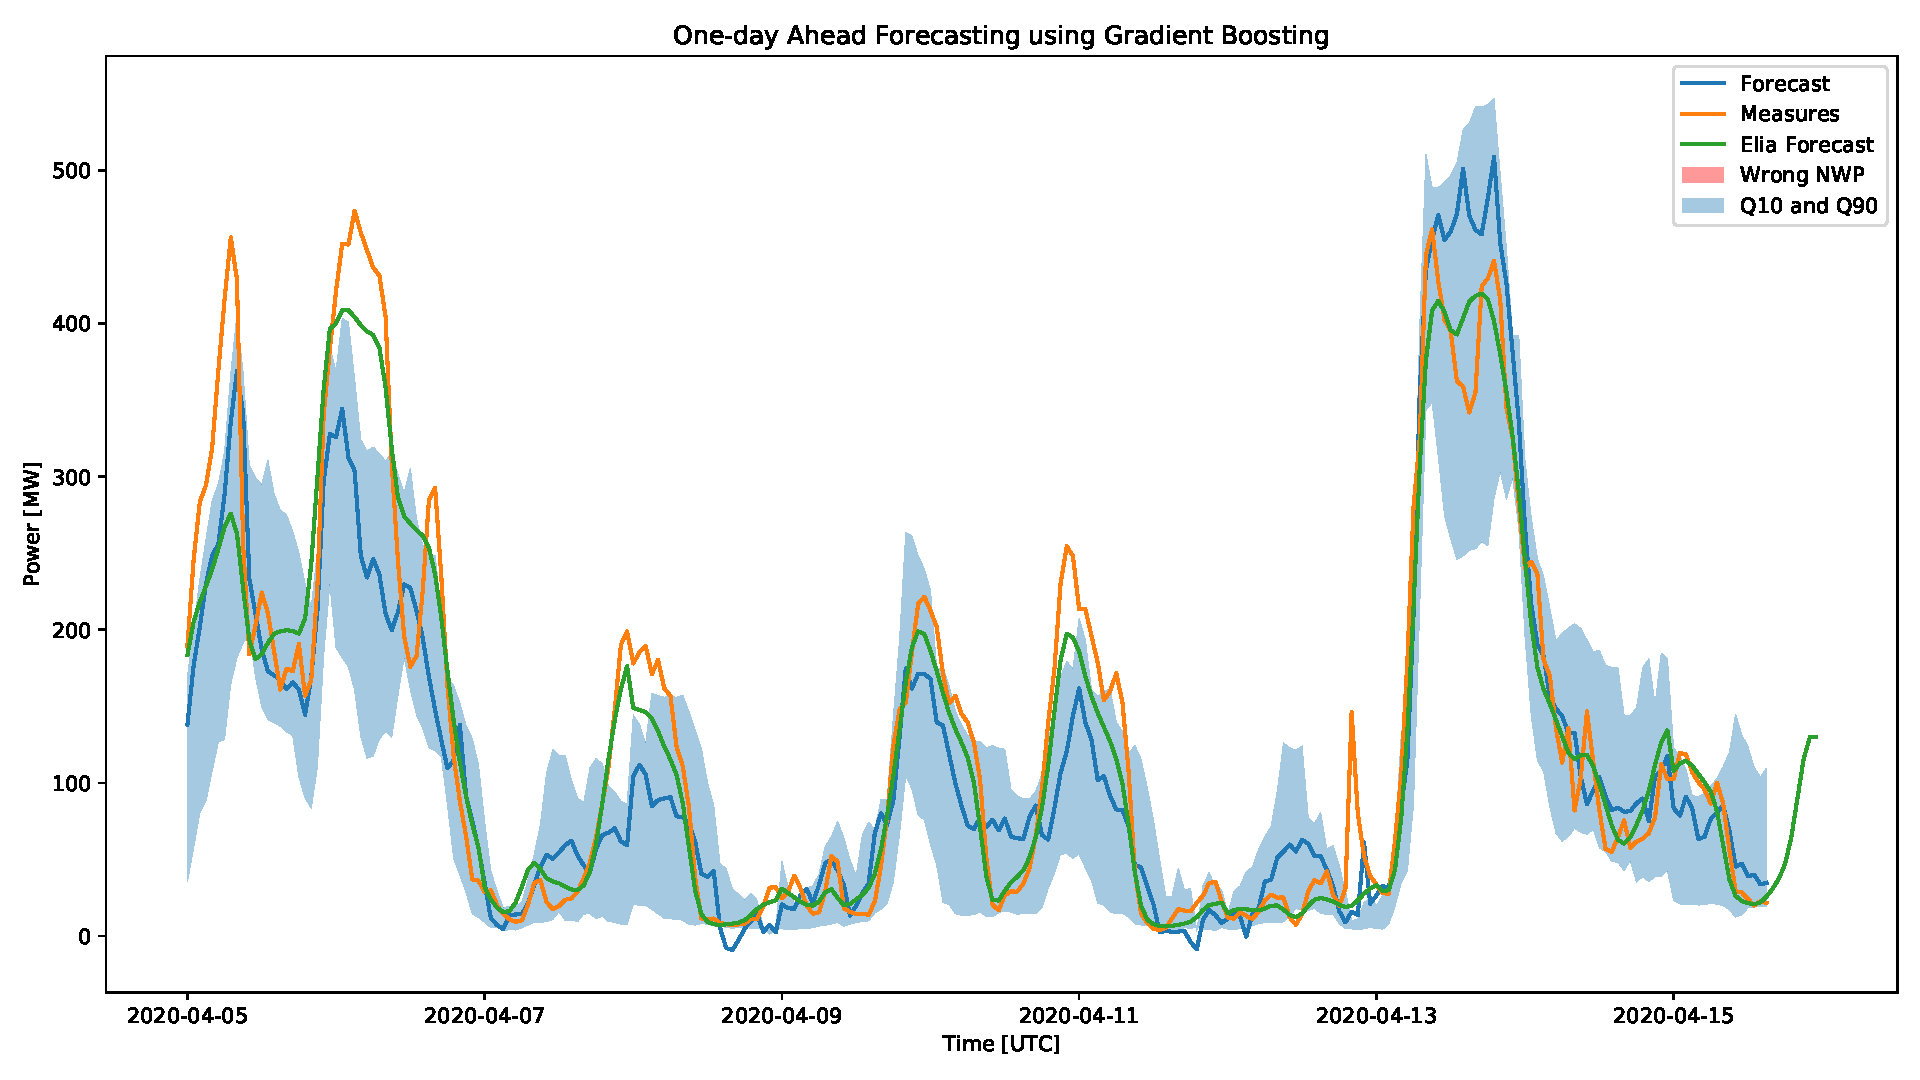
\includegraphics[width=\textwidth]{resources/pdf/odaf68_april.pdf}
        \caption{68-measurements Gradient Boosting}
    \end{subfigure}
    \caption{Comparison of gradient boosting for 15 or 68 measurements}
    \label{fig:wind_test_april}
\end{figure}

For now, we have chosen to keep the model with 68 measurements, as it makes more sense to have the weather measurements at each power plant.

\subsection{Features importance}

Using this last model (Gradient boosting on 68 7-dimensional weather measurements, we have assessed the features importance using their weighted mean impurity reduction along the trees of the gradient boosting method. It yielded the results of figure \ref{fig:featimp} where we can see that, by far, the two most important features were the wind speed and wind gust.

The features are grouped by type (wind speed, wind gust, etc), and the standard deviation along the 68 measurements is colored in blue (Obviously, negative features importance are not possible).

\begin{figure}[H]
    \centering
    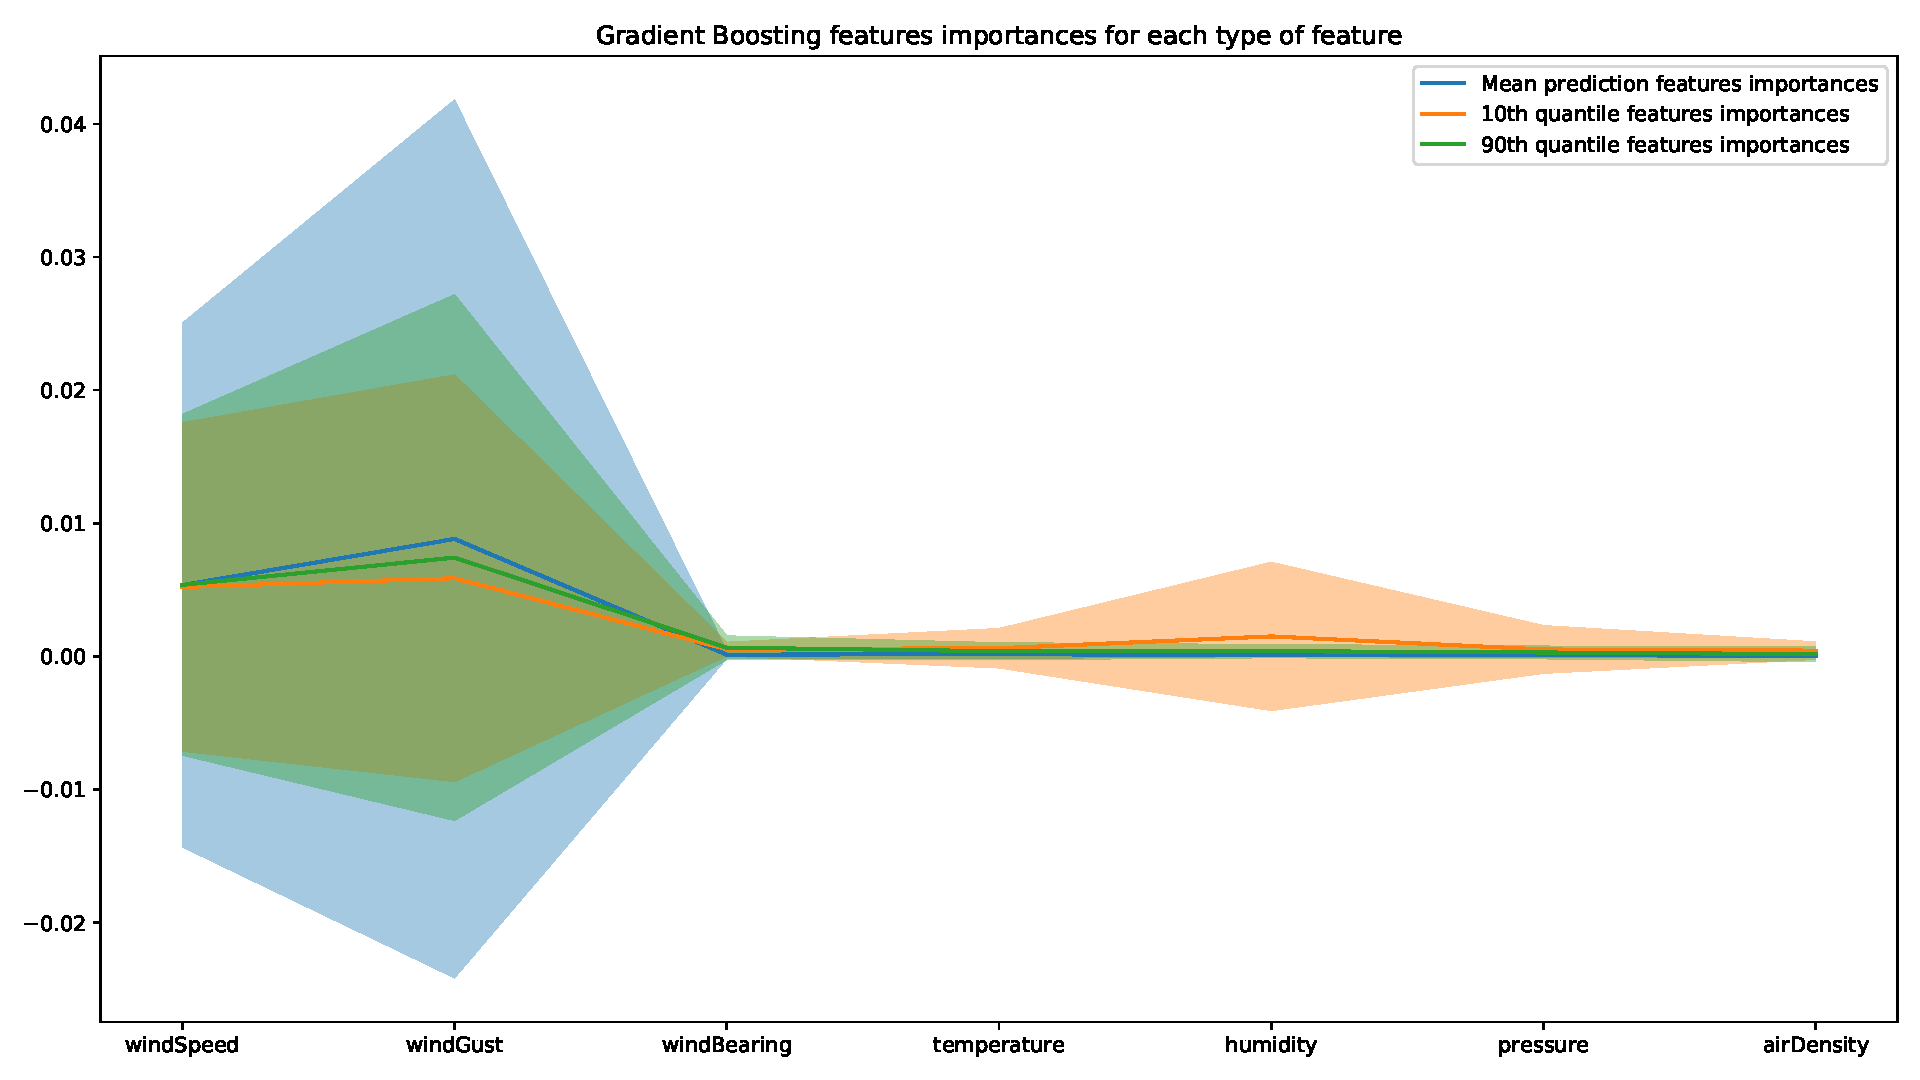
\includegraphics[width=\textwidth]{resources/pdf/fi.pdf}
    \caption{Features Importance}
    \label{fig:featimp}
\end{figure}

Then, we will certainly perform feature selection for the next review, in order to make the model faster to re-train and less prone to overfitting. This should be the only remaining modification brought to the wind forecasting part of the project.
	
\end{document}
